\documentclass[aspectratio=169]{beamer}

\usetheme{default}

% ---------- Packages ----------
\usepackage[utf8]{inputenc}
\usepackage{booktabs}
\usepackage{tabularx}
\usepackage{array}
\usepackage{amsmath}
\usepackage{amssymb}
\usepackage{tikz}
\usepackage{xcolor}
\usepackage{graphicx}
\usepackage{colortbl}
\usepackage{ragged2e}

\usetikzlibrary{positioning,trees,shapes,arrows.meta,calc}
\usepackage{multimedia}

% ============================================================
% PRESENTATION COLOR PALETTE
% ============================================================

\definecolor{maroon}{RGB}{165,0,52}
\definecolor{amritaMaroon}{RGB}{165,0,52}
\definecolor{deepmaroon}{RGB}{145,0,45}
\definecolor{royalblue}{RGB}{0,55,190}

\definecolor{lightblue}{RGB}{220,240,250}
\definecolor{lightgreen}{RGB}{224,245,229}
\definecolor{lightyellow}{RGB}{255,238,205}
\definecolor{lightpink}{RGB}{252,232,238}
\definecolor{lightcyan}{RGB}{222,247,247}
\definecolor{lightorange}{RGB}{255,232,207}
\definecolor{lightpurple}{RGB}{238,231,250}

\definecolor{darktext}{RGB}{35,35,35}

% ============================================================
% GLOBAL BEAMER STYLING
% ============================================================

\setbeamercolor{normal text}{fg=darktext,bg=white}
\setbeamercolor{structure}{fg=maroon}

\setbeamercolor{frametitle}{fg=white,bg=maroon}
\setbeamerfont{frametitle}{size=\large,series=\bfseries}

\setbeamercolor{title}{fg=maroon}
\setbeamercolor{subtitle}{fg=darktext}
\setbeamercolor{author}{fg=darktext}
\setbeamercolor{institute}{fg=darktext}

\setbeamercolor{block title}{fg=white,bg=maroon}
\setbeamercolor{block body}{fg=darktext,bg=lightpink}

\setbeamercolor{alerted text}{fg=maroon}

\setbeamercolor{itemize item}{fg=maroon}
\setbeamercolor{itemize subitem}{fg=maroon}

\setbeamertemplate{navigation symbols}{}

% ============================================================
% FOOTLINE
% ============================================================

\setbeamertemplate{footline}{%
    \leavevmode%
    \hbox{%
        \begin{beamercolorbox}[wd=\paperwidth,ht=0.08cm,dp=0cm]{frametitle}%
        \end{beamercolorbox}%
    }%
}

% ============================================================
% CLEAN HEADER BAR
% ============================================================

\setbeamertemplate{frametitle}{%
    \nointerlineskip%
    \begin{beamercolorbox}[wd=\paperwidth,leftskip=0.5cm,rightskip=0.5cm,vmode]{frametitle}%
        \vskip 0.22cm%
        {\usebeamerfont{frametitle}\insertframetitle\strut\par}%
        \vskip 0.22cm%
    \end{beamercolorbox}%
}

% ============================================================
% HELPER COMMANDS
% ============================================================

\newcommand{\blue}[1]{\textcolor{royalblue}{\textbf{#1}}}
\newcommand{\maroon}[1]{\textcolor{maroon}{\textbf{#1}}}
\newcommand{\tablehead}[1]{\textcolor{white}{\textbf{#1}}}
\newcommand{\coloredtablehead}{\rowcolor{maroon}}

% ============================================================
% TITLE
% ============================================================
\title{
    \textcolor{maroon}{\textbf{Sign Language to 3D Avatar Generation}}
}
\subtitle{
    23CSE399 -- Project Phase 2\\
    Guide Review 1 | Panel Review 1
}
\author{
    Sai Sri Satvic L \\
    Vivin Rakul P \\
    Snigdha Siri Valli A \\
    Vijay Saravana Pandi T
}
\institute{
    \normalsize
    \textbf{Guide: Ms. Nalinadevi K}\\[1mm]
    Department of CSE, Amrita Vishwa Vidyapeetham
}

\date{}

% ============================================================
% DOCUMENT
% ============================================================
\begin{document}

% ============================================================
% TITLE SLIDE
% ============================================================
\begin{frame}[plain]
\vspace*{-0.2cm}
\begin{flushright}
    
\begin{tikzpicture}
        \node[
            fill=maroon, 
            text=white, 
            rounded corners=4pt, 
            inner sep=6pt, 
            font=\small\bfseries
        ] {Type 2: Application Project};
    \end{tikzpicture}
\end{flushright}
\vspace{-1.2cm}
\titlepage
\end{frame}

% ============================================================
% SLIDE 1: MOTIVATION
% ============================================================
\begin{frame}{1. Motivation}
\small
\setbeamertemplate{itemize items}[triangle]

\begin{itemize}
\setlength{\itemsep}{0.15cm}

\item \textcolor{blue}{\textbf{Global Accessibility:}} \textbf{70+ million} deaf and speech-impaired individuals worldwide rely on sign language natively 

\item \textcolor{blue}{\textbf{Linguistic Diversity:}} \textbf{300+ distinct sign languages} exist globally with entirely different grammars

\item \textcolor{blue}{\textbf{Scarcity of Interpreters:}} Critical shortage of certified, affordable interpreters in sectors like healthcare and education

\item \textcolor{blue}{\textbf{Closed-Loop Limitation:}} Predominantly \textbf{video-to-text} translation $\rightarrow$ lacks native visual feedback for the user

\item \textcolor{blue}{\textbf{Translation Bottleneck:}} Absence of a shared phonetic intermediate representation prevents universal translation

\end{itemize}
\end{frame}

% ============================================================
% SLIDE 2: INTRODUCTION
% ============================================================
\section{Introduction}
\begin{frame}{2. Introduction}
\small
\setlength{\itemsep}{8pt}

\begin{itemize}
\item \textcolor{blue}{\textbf{Motion Tracking:}} \textit{What is happening?} $\rightarrow$ Hand moving up, fingers bending.
\item \textcolor{blue}{\textbf{Linguistic Meaning:}} \textit{Why is it happening?} $\rightarrow$ Flat Hand + Pointing Up $\rightarrow$ Sign for ``Hello''.
\item \textcolor{blue}{\textbf{Movement $\neq$ Meaning:}} The same physical gesture can mean \textbf{different things} depending on context.
\item \textcolor{blue}{\textbf{Real-World Complexity:}} 3D rotations + varying camera depths + \textbf{noisy data} make translation harder to infer.
\item \textcolor{blue}{\textbf{Beyond Basic Tracking:}} Understanding \textbf{exact handshapes, orientations, and 3D depth} enables true linguistic translation.
\item \textcolor{blue}{\textbf{Our Goal:}} Move from \textbf{raw landmark tracking} $\rightarrow$ \textbf{3D anatomical modeling} $\rightarrow$ \textbf{accurate sign translation}.
\end{itemize}
\end{frame}

% ============================================================
% SLIDE 3: LITERATURE SURVEY PART 1
% ============================================================
\section{Literature Survey}
\begin{frame}{3. Literature Survey: Sign Language Translation (Part 1)}
\begin{table}
\centering
\renewcommand{\arraystretch}{1.3}
\scriptsize
\begin{tabular}{|p{3.0cm}|c|p{4.5cm}|p{4.5cm}|}
\hline
\rowcolor{maroon}
\textcolor{white}{\textbf{Authors}} & \textcolor{white}{\textbf{Year}} & \textcolor{white}{\textbf{Key Contribution}} & \textcolor{white}{\textbf{Limitation}} \\
\hline
\rowcolor{lightblue}
\textbf{Kaur \& Kumar} & 2016 & HamNoSys $\rightarrow$ SiGML conversion for ISL animation & Only isolated signs, manual annotation required. \\
\hline
\rowcolor{lightgreen}
\textbf{Saunders et al.} & 2020 & SignGAN: speech $\rightarrow$ photorealistic sign video & High computational cost, needs large annotated datasets. \\
\hline
\rowcolor{lightcyan}
\textbf{Goyal et al.} & 2020 & Grammar-based English $\rightarrow$ ISL animation & Rule-dependent, not scalable, ambiguity issues. \\
\hline
\rowcolor{lightorange}
\textbf{Skobov \& Lepage} & 2020 & Video $\rightarrow$ HamNoSys automatic annotation & Accuracy affected by video quality, finger/facial capture limited. \\
\hline
\rowcolor{lightpurple}
\textbf{Shalev-Arkushin et al.} & 2022 & HamNoSys $\rightarrow$ 3D pose sequences & Needs HamNoSys expertise, coarticulation handling difficult. \\
\hline
\end{tabular}
\end{table}

\vspace{0.15cm}
\centering
\fcolorbox{maroon}{lightpink}{
\begin{minipage}{0.95\textwidth}
\footnotesize

\end{minipage}
}
\end{frame}

% ============================================================
% SLIDE 4: LITERATURE SURVEY PART 2
% ============================================================
\begin{frame}{4. Literature Survey: Sign Language Translation (Part 2)}
\begin{table}
\centering
\renewcommand{\arraystretch}{1.3}
\scriptsize
\begin{tabular}{|p{3.0cm}|c|p{4.5cm}|p{4.5cm}|}
\hline
\rowcolor{maroon}
\textcolor{white}{\textbf{Authors}} & \textcolor{white}{\textbf{Year}} & \textcolor{white}{\textbf{Key Contribution}} & \textcolor{white}{\textbf{Limitation}} \\
\hline
\rowcolor{lightblue}
\textbf{Forte et al.} & 2023 & Linguistic priors + deep learning for video $\rightarrow$ avatar & Requires extensive linguistic modeling, high-quality videos. \\
\hline
\rowcolor{lightgreen}
\textbf{Yu et al.} & 2023 & SignAvatars dataset: large-scale 3D motion & Limited language coverage, facial expressions challenging. \\
\hline
\rowcolor{lightcyan}
\textbf{Gil-Mart\'{\i}n et al.} & 2023 & Motion generation from linguistic features & Needs accurate annotations, hard to scale to continuous signing. \\
\hline
\rowcolor{lightorange}
\textbf{Villa-Monedero et al.} & 2023 & Dataset for motion generation & Limited size \& coverage. \\
\hline
\rowcolor{lightpurple}
\textbf{Krishnamurthy et al.} & 2024 & DiffSign: diffusion model for customizable sign videos & Computationally heavy, dataset scarcity. \\
\hline
\end{tabular}
\end{table}

\vspace{0.15cm}
\centering
\fcolorbox{maroon}{lightpink}{
\begin{minipage}{0.95\textwidth}
\footnotesize

\end{minipage}
}
\end{frame}

% ============================================================
% SLIDE 6: PROBLEM STATEMENT
% ============================================================
\section{Problem Statement}
\begin{frame}{5. Problem Statement}
\vspace{0.3cm}
\centering
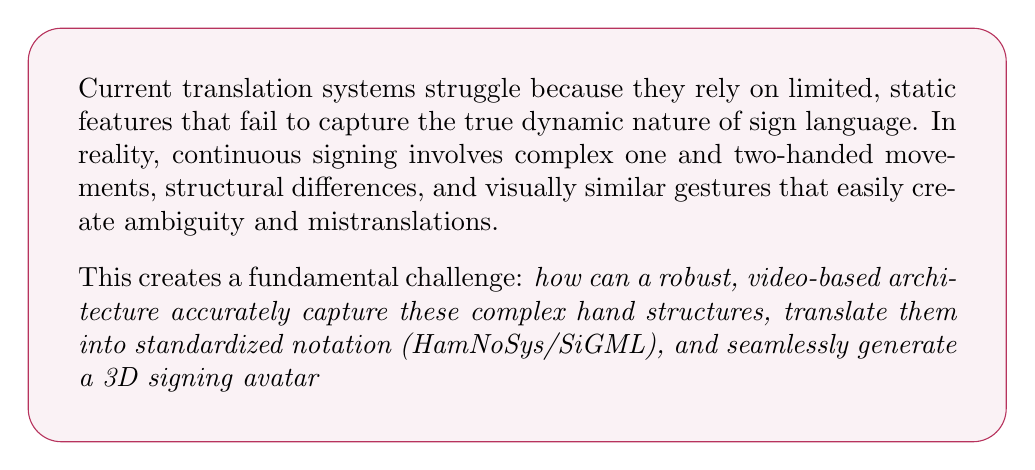
\begin{tikzpicture}
\node[
    draw=amritaMaroon!80,
    fill=amritaMaroon!5,
    rounded corners=12pt,
    inner sep=18pt,
    text width=0.92\textwidth,
    align=justify
]
{
Current translation systems struggle because they rely on limited, static features that fail to capture the true dynamic nature of sign language. In reality, continuous signing involves complex one and two-handed movements, structural differences, and visually similar gestures that easily create ambiguity and mistranslations.

\vspace{0.3cm}
This creates a fundamental challenge:
\textit{how can a robust, video-based architecture accurately capture these complex hand structures, translate them into standardized notation (HamNoSys/SiGML), and seamlessly generate a 3D signing avatar}
};
\end{tikzpicture}
\end{frame}

% ============================================================
% SLIDE 7: RESEARCH OBJECTIVES
% ============================================================
\begin{frame}{6. Research Objectives}
\footnotesize
\begin{itemize}
\setlength{\itemsep}{0.16cm}
\item \textbf{RO1:} To build a complete video-to-avatar system that takes sign language videos as input and generates 3D avatar animations using HamNoSys as a universal intermediate representation.
\item \textbf{RO2:} To accurately classify the 6 fundamental components of a sign --- Handshape, Finger Direction, Palm Orientation, Body Location, Movement, and Two-Handed Structure .
\item \textbf{RO3:} To ensure linguistic correctness by developing a grammar compiler that validates every generated HamNoSys sequence before avatar rendering.
\item \textbf{RO4:} To automate the entire pipeline from video input to avatar output, eliminating the need for manual annotation or intervention at any stage.
\item \textbf{RO5:} To establish a foundation for cross-sign-language translation, proving that HamNoSys can serve as a universal bridge between different sign languages (e.g., ASL to ISL).
\end{itemize}
\end{frame}

% ============================================================
% SLIDE 8: SYSTEM ARCHITECTURE
% ============================================================
\section{System Architecture}
\begin{frame}{7. System Architecture}
\centering
\vspace{-0.2cm}
\includegraphics[
    width=\textwidth,
    height=0.88\textheight,
    keepaspectratio
]{updated_archi.png}
\end{frame}

% ============================================================
% SLIDE 8: ARCHITECTURE EVOLUTION
% ============================================================
\section{Architecture Evolution}
\begin{frame}{8. Architecture Evolution: Old vs New Pipeline}
\centering
\vspace{-1mm}
{\small\itshape The major implementation change in the current phase}
\vspace{1.5mm}

\begin{columns}[T]
\column{0.48\textwidth}
\centering
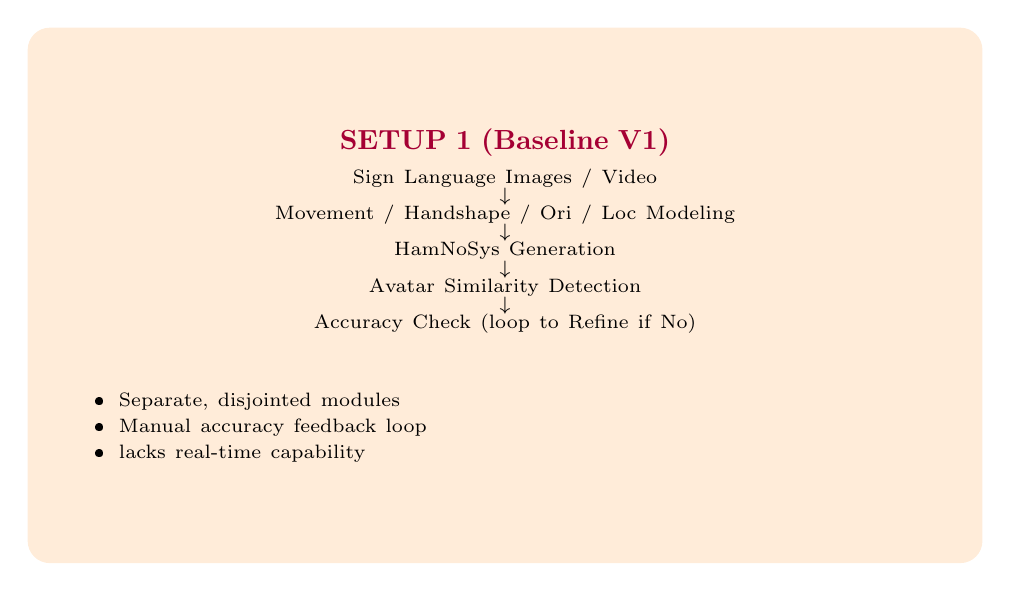
\begin{tikzpicture}
\node[
    fill=orange!15,
    rounded corners=8pt,
    inner sep=8pt,
    text width=\columnwidth-16pt,
    align=center,
    minimum height=6.8cm
]
{
{\bfseries\textcolor{amritaMaroon}{\normalsize SETUP 1 (Baseline V1)}}\\[1.5mm]
\scriptsize
Sign Language Images / Video \\[-0.5mm]
$\downarrow$ \\[-0.5mm]
Movement / Handshape / Ori / Loc Modeling \\[-0.5mm]
$\downarrow$ \\[-0.5mm]
HamNoSys Generation \\[-0.5mm]
$\downarrow$ \\[-0.5mm]
Avatar Similarity Detection \\[-0.5mm]
$\downarrow$ \\[-0.5mm]
Accuracy Check (loop to Refine if No)

\vspace{3.5mm}
\raggedright
\begin{itemize}
\setlength{\itemsep}{1.5pt}
\setlength{\parskip}{0pt}
\item Separate, disjointed modules
\item Manual accuracy feedback loop
\item lacks real-time capability
\end{itemize}
};
\end{tikzpicture}

\column{0.48\textwidth}
\centering
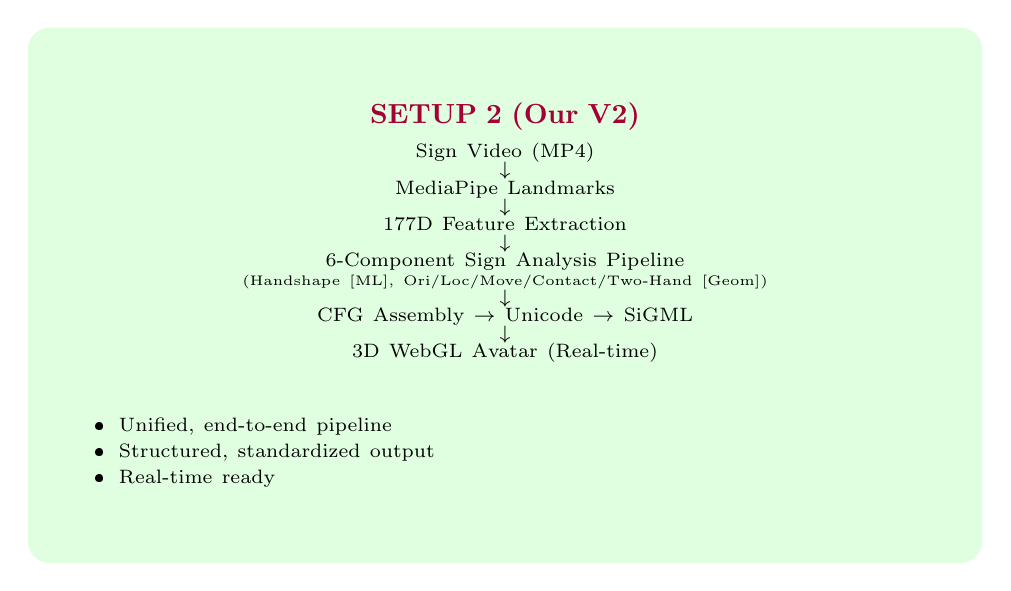
\begin{tikzpicture}
\node[
    fill=green!12,
    rounded corners=8pt,
    inner sep=8pt,
    text width=\columnwidth-16pt,
    align=center,
    minimum height=6.8cm
]
{
{\bfseries\textcolor{amritaMaroon}{\normalsize SETUP 2 (Our V2)}}\\[1.5mm]
\scriptsize
Sign Video (MP4) \\[-0.5mm]
$\downarrow$ \\[-0.5mm]
MediaPipe Landmarks \\[-0.5mm]
$\downarrow$ \\[-0.5mm]
177D Feature Extraction \\[-0.5mm]
$\downarrow$ \\[-0.5mm]
6-Component Sign Analysis Pipeline \\[-0.5mm]
{\tiny (Handshape [ML], Ori/Loc/Move/Contact/Two-Hand [Geom])} \\[-0.5mm]
$\downarrow$ \\[-0.5mm]
CFG Assembly $\to$ Unicode $\to$ SiGML \\[-0.5mm]
$\downarrow$ \\[-0.5mm]
3D WebGL Avatar (Real-time)

\vspace{3mm}
\raggedright
\begin{itemize}
\setlength{\itemsep}{1.5pt}
\setlength{\parskip}{0pt}
\item Unified, end-to-end pipeline
\item Structured, standardized output
\item Real-time ready
\end{itemize}
};
\end{tikzpicture}
\end{columns}

\vspace{2mm}
% Added 177D Explanation Box (Phase 5)
\centering
\fcolorbox{amritaMaroon}{white}{
    \parbox{0.95\textwidth}{
        \centering \scriptsize \textbf{*What is the 177D Tensor?} \\
        It combines normalized hand and selected upper-body landmark coordinates into a fixed-size feature vector used by the downstream analysis modules.
    }
}
\end{frame}

% ============================================================
% SLIDE 8a: DUAL-PATH SYSTEM ARCHITECTURE
% ============================================================
\begin{frame}[t]{8a. Dual-Path Architecture: Production Deployed vs. Neural Network}
\vspace{-0.1cm}
\begin{center}
    \scriptsize\textit{\textcolor{amritaMaroon}{Two independent execution paths designed for distinct operational objectives}}
\end{center}

\vspace{-1.5mm}
\begin{columns}[T]
    \column{0.49\textwidth}
    \setbeamercolor{block title}{fg=white,bg=maroon}
    \setbeamercolor{block body}{fg=darktext,bg=lightblue}
    \begin{block}{Path A: Production Deployed Pipeline}
        \fontsize{6.8pt}{8.6pt}\selectfont
        \textbf{Pipeline Flow:}
        \begin{itemize}\setlength{\itemsep}{1.2pt}
            \item \textbf{Input:} MP4 Video (30 fps, $\sim$150 frames)
            \item \textbf{Landmarks:} MediaPipe 177D normalized coordinates
            \item \textbf{Feature Extraction:} 10 Parallel Heuristic / ML Modules (Handshape ML + Zero-Shot Vector Geometry)
            \item \textbf{Noise Filtering:} Temporal Phase Segmentation (15--50\%, 55--100\%) \& Statistical Majority Voting
            \item \textbf{Grammar Assembly:} \textbf{CFG Compiler} (strict BNF rules)
            \item \textbf{Rendering:} SiGML XML $\to$ Real-Time WebGL 3D Avatar
        \end{itemize}
        \vspace{1mm}
        \textbf{Status:} \textcolor{green!60!black}{\textbf{Live in Production}} (Powers Flask webapp; 85.7\% precision across 170 ASL benchmark glosses).
    \end{block}

    \column{0.49\textwidth}
    \setbeamercolor{block title}{fg=white,bg=maroon}
    \setbeamercolor{block body}{fg=darktext,bg=lightgreen}
    \begin{block}{Path B: Deep Learning Sequence Model}
        \fontsize{6.8pt}{8.6pt}\selectfont
        \textbf{Pipeline Flow:}
        \begin{itemize}\setlength{\itemsep}{1.2pt}
            \item \textbf{Input:} 177D Landmarks $\times$ 150 frames sequence tensor
            \item \textbf{Local Features:} 1D-CNN (Temporal Conv1D, BatchNorm, ReLU)
            \item \textbf{Sequence Modeling:} \textbf{2-Layer BiGRU} (bidirectional past and future temporal context, 128 hidden)
            \item \textbf{Aggregation:} Temporal Attention Pooling (learns frame weights)
            \item \textbf{Prediction:} 6 Multi-Task Classification Heads
            \item \textbf{Optimization:} Joint multi-task cross-entropy loss
        \end{itemize}
        \vspace{1mm}
        \textbf{Status:} \textcolor{blue!80!black}{\textbf{Research Prototype}} (eliminates heuristic threshold tuning; 360$\times$ smaller than senior 290M model).
    \end{block}
\end{columns}

\vspace{1.5mm}
\centering
\fcolorbox{amritaMaroon}{lightyellow}{
    \parbox{0.96\textwidth}{
        \fontsize{6.5pt}{8.2pt}\selectfont
        \textbf{Key Architectural Insight:} The two paths do \textbf{not} cancel each other out. The heuristic+CFG pipeline provides immediate, mathematically proven grammatical stability for deployment, while the BiGRU eliminates manual threshold fragility through learned spatio-temporal representations.
    }
}
\end{frame}


% ============================================================
% SLIDE 9: DATASET
% ============================================================
\section{Dataset and Feature Architecture}
\begin{frame}{9. Dataset explanation}
\small
\begin{columns}[c]
\column{0.65\textwidth}
\textbf{WLASL Dataset}
\begin{itemize}
\item \textbf{Large-scale ASL Dataset:} WLASL contains around \textbf{21,000 videos} covering \textbf{2,000 isolated ASL glosses}.
\item \textbf{Real-World Diversity:} Videos contain different signers, backgrounds, lighting conditions, camera angles, resolutions, and signing speeds.
\item \textbf{Different Sign Structures:} The dataset includes \textbf{one-handed and two-handed signs}, allowing the system to learn different signing patterns.
\item \textbf{Robustness:} This diversity reduces overfitting to a particular signer or environment and improves performance on \textbf{live webcam inputs}.
\end{itemize}

\column{0.35\textwidth}
\centering
\includegraphics[
    width=\textwidth,
    keepaspectratio
]{image_1.png}
\end{columns}
\end{frame}

% ============================================================
% SLIDE 10: FEATURE EXTRACTION PIPELINE
% ============================================================
\section{Feature Extraction}
\begin{frame}{10. Feature Extraction \& 177D Representation}
    \centering
    \vspace{1mm}
    
    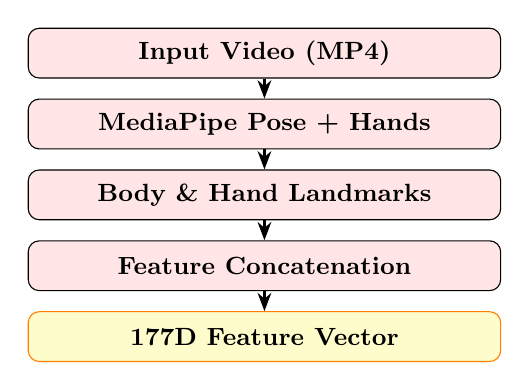
\begin{tikzpicture}[
        block/.style={rectangle, draw=black, fill=red!10, text=black, font=\bfseries\small, align=center, rounded corners=4pt, minimum height=1.8em, minimum width=6cm, inner sep=3pt},
        arrow/.style={-{Stealth[scale=1.0]}, thick, black}
    ]
        % Tighter spacing to prevent overflow
        \node (input) at (0, 0) [block] {Input Video (MP4)};
        \node (mp) at (0, -0.9) [block] {MediaPipe Pose + Hands};
        \node (landmarks) at (0, -1.8) [block] {Body \& Hand Landmarks};
        \node (concat) at (0, -2.7) [block] {Feature Concatenation};
        \node (tensor) at (0, -3.6) [block, fill=yellow!20, draw=orange] {177D Feature Vector};
        
        \draw [arrow] (input) -- (mp);
        \draw [arrow] (mp) -- (landmarks);
        \draw [arrow] (landmarks) -- (concat);
        \draw [arrow] (concat) -- (tensor);
    \end{tikzpicture}
    
    \vspace{4mm}
    \fcolorbox{black}{white}{
        \parbox{0.85\textwidth}{
            \centering \small \textbf{What is the 177D Vector?} \\
            \vspace{1mm}
            \footnotesize
            The 177D representation combines normalized hand and selected upper-body landmark coordinates into a fixed-size feature vector. This single tensor is passed downstream to all analysis modules.
        }
    }
\end{frame}


% ============================================================
% SLIDE 11: SIGN ANALYSIS PIPELINE
% ============================================================
\section{Sign Analysis Modules}
\begin{frame}{11. Six-Component Sign Analysis Pipeline}
    \centering
    \vspace{-1mm}
    
    
    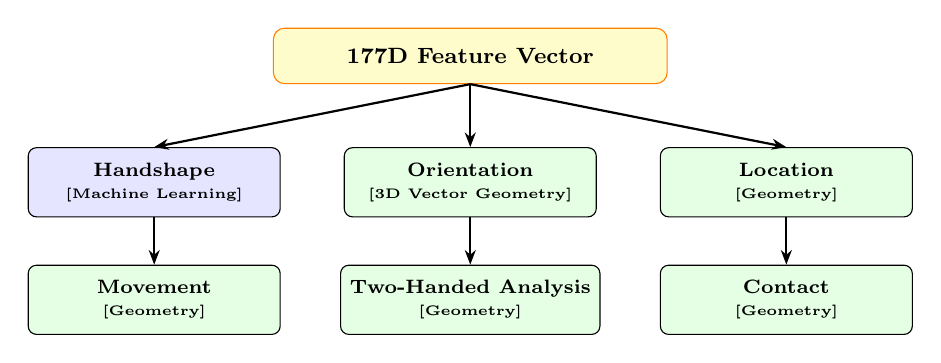
\begin{tikzpicture}[
        node distance=0.5cm and 0.8cm,
        mlblock/.style={rectangle, draw=black, fill=blue!10, text=black, font=\bfseries\scriptsize, align=center, rounded corners=3pt, minimum height=2.5em, minimum width=3.2cm},
        geomblock/.style={rectangle, draw=black, fill=green!10, text=black, font=\bfseries\scriptsize, align=center, rounded corners=3pt, minimum height=2.5em, minimum width=3.2cm},
        titleblock/.style={rectangle, draw=orange, fill=yellow!20, text=black, font=\bfseries\footnotesize, align=center, rounded corners=4pt, minimum height=2em, minimum width=5cm},
        arrow/.style={-{Stealth[scale=0.8]}, thick, black}
    ]
        
        % Top Node
        \node (title) [titleblock] {177D Feature Vector};
        
        % Layer 1
        \node (ori) [geomblock, below=0.8cm of title] {Orientation\\{\tiny [3D Vector Geometry]}};
        \node (hs) [mlblock, left=of ori] {Handshape\\{\tiny [Machine Learning]}};
        \node (loc) [geomblock, right=of ori] {Location\\{\tiny [Geometry]}};
        
        % Layer 2
        \node (twohand) [geomblock, below=0.6cm of ori] {Two-Handed Analysis\\{\tiny [Geometry]}};
        \node (mov) [geomblock, below=0.6cm of hs] {Movement\\{\tiny [Geometry]}};
        \node (contact) [geomblock, below=0.6cm of loc] {Contact\\{\tiny [Geometry]}};
        
        % Safe routing from title 
        \draw [arrow] (title.south) -- (hs.north);
        \draw [arrow] (title.south) -- (ori.north);
        \draw [arrow] (title.south) -- (loc.north);
        
        % Routing to layer 2 (downward flow)
        \draw [arrow] (hs.south) -- (mov.north);
        \draw [arrow] (ori.south) -- (twohand.north);
        \draw [arrow] (loc.south) -- (contact.north);
        
    \end{tikzpicture}
    
    \vspace{4mm}
    \begin{columns}[T]
        \column{0.45\textwidth}
        \begin{block}{Machine Learning Module}
            \scriptsize
            \textbf{Handshape:} Our only ML classifier. Evaluates joint angles to classify shapes (trained on augmented dataset).
        \end{block}
        
        \column{0.5\textwidth}
        \begin{block}{Zero-Shot Geometry (Orientation)}
            \scriptsize
            \textbf{Palm Orientation Calculation:} \\
            MediaPipe Landmarks $\to$ 3D Vector Geometry $\to$ Cross Product $\to$ Palm Normal $\to$ Palm Orientation.
        \end{block}
    \end{columns}
\end{frame}

% ============================================================
% SLIDE 11a: DEEP LEARNING SEQUENCE ARCHITECTURE (BiGRU)
% ============================================================
\begin{frame}[t]{11a. Deep Learning Architecture: 1D-CNN + BiGRU + Attention}
\vspace{-0.1cm}
\begin{center}
    \scriptsize\textit{\textcolor{amritaMaroon}{Capturing spatio-temporal gesture dynamics across 150 frames without hand-crafted thresholds}}
\end{center}

\vspace{-1.5mm}
\begin{columns}[T]
    \column{0.49\textwidth}
    \setbeamercolor{block title}{fg=white,bg=maroon}
    \setbeamercolor{block body}{fg=darktext,bg=lightyellow}
    \begin{block}{Temporal vs. Non-Temporal Modeling}
        \fontsize{6.8pt}{8.6pt}\selectfont
        \textbf{Non-Temporal (Single Frame):}
        \begin{itemize}\setlength{\itemsep}{1pt}
            \item Instantaneous landmark coordinates $(x, y, z)$.
            \item Static hand posture (e.g., fist, flat hand).
            \item Cannot distinguish movement direction (e.g., upward vs downward) at apex frames.
        \end{itemize}
        \vspace{1mm}
        \textbf{Temporal (BiGRU Hidden States):}
        \begin{itemize}\setlength{\itemsep}{1pt}
            \item Forward $\overrightarrow{h}_t$: Past trajectory context (where hand originated).
            \item Backward $\overleftarrow{h}_t$: Anticipatory future context (where hand terminates).
            \item Automatically learns velocity, acceleration, and state transitions without manual velocity thresholds.
        \end{itemize}
    \end{block}

    \column{0.49\textwidth}
    \setbeamercolor{block title}{fg=white,bg=maroon}
    \setbeamercolor{block body}{fg=darktext,bg=lightblue}
    \begin{block}{HamNoSysSequenceNet Architecture}
        \fontsize{6.8pt}{8.6pt}\selectfont
        \textbf{Layer-by-Layer Tensor Flow:}
        \begin{itemize}\setlength{\itemsep}{1.2pt}
            \item \textbf{Input Tensor:} $(B, T=150, D=177)$
            \item \textbf{1D-CNN:} $\text{Conv1D}(177 \to 128) \to \text{BN} \to \text{ReLU} \to \text{Conv1D}(128 \to 128)$
            \item \textbf{BiGRU:} 2-layer Bidirectional GRU (hidden=64, bidirectional $\to$ 128-dim per frame)
            \item \textbf{Attention Pooling:} $\alpha_t = \text{Softmax}(w^T \tanh(W h_t))$ computes frame importance weights
            \item \textbf{6 Multi-Task Heads:}
                  $\text{FC}_{\text{hs}}(11), \text{FC}_{\text{ext}}(3), \text{FC}_{\text{palm}}(3), \text{FC}_{\text{loc}}(8), \text{FC}_{\text{mov}}(8), \text{FC}_{\text{two}}(3)$
        \end{itemize}
        \vspace{1mm}
        \textbf{Efficiency:} Only \textbf{0.8M parameters} (vs. seniors' 290M VGG16), trained on unified ISL landmark sequences.
    \end{block}
\end{columns}

\vspace{1.5mm}
\centering
\fcolorbox{amritaMaroon}{white}{
    \parbox{0.96\textwidth}{
        \centering\fontsize{6.5pt}{8.2pt}\selectfont
        \textbf{Advantage over Senior Pipeline:} Replaces brittle hand-tuned heuristics with end-to-end learned sequence representations that generalize across diverse signers and camera framings.
    }
}
\end{frame}

% ============================================================
% SLIDE 12: FORMAL 4-TUPLE GRAMMAR SPECIFICATION
% ============================================================
\section{CFG Grammar Compiler}
\begin{frame}[t]{12. Context-Free Grammar: Formal 4-Tuple Specification}
\vspace{-0.1cm}
\begin{center}
    \scriptsize\textit{\textcolor{amritaMaroon}{Formal theoretical definition $G = (V, T, P, S)$ and project mapping (Hopcroft et al., 2006)}}
\end{center}

\vspace{-1.5mm}
\setbeamercolor{block title}{fg=white,bg=maroon}
\setbeamercolor{block body}{fg=darktext,bg=lightpink}
\begin{block}{Theoretical Role: Lexer vs. Parser Architecture}
    \fontsize{6.8pt}{8.6pt}\selectfont
    The feature extraction pipeline (BiGRU / 10 heuristic modules) acts as the \textbf{Lexer} (producing unconstrained phonetic probabilities). The CFG compiler acts as the \textbf{Parser} (enforcing strict phonological syntax), converting chaotic predictions into a deterministic HamNoSys sequence for 3D avatar execution.
\end{block}

\vspace{1.2mm}
\centering
\setlength{\tabcolsep}{4pt}
\renewcommand{\arraystretch}{1.22}
{\fontsize{6.8pt}{8.6pt}\selectfont
\begin{tabular}{|>{\centering\arraybackslash\bfseries}p{0.8cm}|>{\raggedright\arraybackslash\bfseries}p{2.3cm}|>{\raggedright\arraybackslash}p{6.4cm}|>{\raggedright\arraybackslash}p{3.0cm}|}
    \hline
    \rowcolor{maroon}
    \textcolor{white}{\textbf{Tuple}} & 
    \textcolor{white}{\textbf{Grammar Component}} & 
    \textcolor{white}{\textbf{Formal Mathematical Definition \& Disjoint Alphabet}} & 
    \textcolor{white}{\textbf{Role in SignBridge V2}} \\
    \hline
    \rowcolor{lightblue} 
    $V$ & Variables / Non-Terminals ($|V|=17$) & 
    $V = \{\langle\text{Sign}\rangle, \langle\text{ManualConfig}\rangle, \langle\text{Symmetry}\rangle, \langle\text{SingleHand}\rangle, \langle\text{DualHand}\rangle, \langle\text{Orientation}\rangle, \langle\text{Handshape}\rangle, \dots\}$ & 
    Syntactic categories mapping to Stokoe's Tab-Dez-Sig phonological constituents. \\
    \hline
    \rowcolor{lightgreen} 
    $T$ & Terminals / Alphabet ($|T|=83$) & 
    \textbf{Disjoint Partition Alphabet:}\\[0.5mm]
    $\mathbf{T = \bigsqcup_{k=1}^8 T_k = T_{\text{symm}} \sqcup T_{\text{hs}} \sqcup T_{\text{ext}} \sqcup T_{\text{palm}} \sqcup T_{\text{loc}} \sqcup T_{\text{cont}} \sqcup T_{\text{mov}} \sqcup T_{\text{trans}}}$\\[0.5mm]
    $\bullet\; T_{\text{symm}} (3):\; \{\texttt{hamsymmlr}, \texttt{hamnonipsi}, \texttt{hamplus}\}$\\[0.2mm]
    $\bullet\; T_{\text{hs}} (20):\; \text{Handshapes } \{\texttt{hamflathand}, \texttt{hamfist}, \dots\}$\\[0.2mm]
    $\bullet\; T_{\text{ext}} (10):\; \text{Extended fingers } \{\texttt{hamextfingeru}, \dots\}$\\[0.2mm]
    $\bullet\; T_{\text{palm}} (8):\; \text{Palm facings } \{\texttt{hampalmu}, \texttt{hampalmd}, \dots\}$\\[0.2mm]
    $\bullet\; T_{\text{loc}} (25):\; \text{Body locations } \{\texttt{hamchest}, \texttt{hamhead}, \dots\}$\\[0.2mm]
    $\bullet\; T_{\text{cont}} (4):\; \text{Contact types } \{\texttt{hamtouch}, \texttt{hamclose}, \dots\}$\\[0.2mm]
    $\bullet\; T_{\text{mov}} (12):\; \text{Movements } \{\texttt{hammoveo}, \texttt{hamcircle}, \dots\}$\\[0.2mm]
    $\bullet\; T_{\text{trans}} (1):\; \text{Dynamic posture replace } \{\texttt{hamreplace}\}$ & 
    83 atomic HamNoSys phonetic tokens driving WebGL avatar bone rotations. \\
    \hline
    \rowcolor{lightyellow} 
    $P$ & Production Rules ($|P|=17$) & 
    Rewriting rules in Backus-Naur Form (BNF): $A \to \alpha$, where $A \in V$ and $\alpha \in (V \cup T)^*$ & 
    Enforces linear syntax order: $\text{Hand} \to \text{Loc} \to \text{Contact} \to \text{Movement}$. \\
    \hline
    \rowcolor{lightorange} 
    $S$ & Start Symbol & 
    $S = \langle\text{Sign}\rangle \in V$ & 
    Root sentence symbol representing the complete gesture derivation. \\
    \hline
\end{tabular}
}

\vspace{1.2mm}
\fcolorbox{amritaMaroon}{white}{
    \parbox{0.96\textwidth}{
        \centering\fontsize{6.4pt}{8.0pt}\selectfont
        \textbf{Formal Language Guarantee:} The generated sign language $L(G) = \{w \in T^* \mid S \implies^* w\}$ is guaranteed to be context-free and parseable by the CWASA WebGL SiGML engine without runtime ambiguity.
    }
}
\end{frame}

% ============================================================
% SLIDE 12a-1: FORMAL CFG PRODUCTION RULES (CORE BACKBONE)
% ============================================================
\begin{frame}[t]{12a. Formal CFG Production Rules: Core Structural Backbone}
\vspace{-0.1cm}
\begin{center}
    \scriptsize\textit{\textcolor{amritaMaroon}{Linguistically grounded rewrite rules enforcing strict phonological ordering (Rules P1--P5)}}
\end{center}

\vspace{-1.5mm}
\centering
\setlength{\tabcolsep}{4pt}
\renewcommand{\arraystretch}{1.28}
{\fontsize{7.2pt}{9.2pt}\selectfont
\begin{tabular}{|>{\centering\arraybackslash\bfseries}p{1.0cm}|>{\raggedright\arraybackslash\bfseries}p{2.6cm}|>{\raggedright\arraybackslash}p{5.8cm}|>{\raggedright\arraybackslash}p{3.2cm}|}
    \hline
    \rowcolor{maroon}
    \textcolor{white}{\textbf{Rule ID}} & 
    \textcolor{white}{\textbf{Constituent Name}} & 
    \textcolor{white}{\textbf{Production Rule in Backus-Naur Form (BNF)}} & 
    \textcolor{white}{\textbf{Linguistic Meaning \& Scope}} \\
    \hline
    \rowcolor{lightblue} 
    \textbf{P1} & Root Sign & 
    $\langle\text{Sign}\rangle \to \langle\text{ManualConfig}\rangle \;\mid\; \langle\text{Symmetry}\rangle \;\langle\text{ManualConfig}\rangle$ & 
    Top-level sentence expansion with optional bilateral symmetry prefix. \\
    \hline
    \rowcolor{lightgreen} 
    \textbf{P2} & Manual Configuration & 
    $\langle\text{ManualConfig}\rangle \to \langle\text{SingleHand}\rangle \;\langle\text{Location}\rangle \;[\langle\text{Contact}\rangle] \;[\langle\text{Movement}\rangle] \;[\langle\text{StateTransition}\rangle]$ & 
    Core linear sign syntagm: Hand posture followed by body anchor and optional modifiers. \\
    \hline
    \rowcolor{lightyellow} 
    \textbf{P3} & Single-Hand Form & 
    $\langle\text{SingleHand}\rangle \to \langle\text{Handshape}\rangle \;\langle\text{Orientation}\rangle$ & 
    Phonological hand unit combining anatomical handshape and 3D spatial attitude. \\
    \hline
    \rowcolor{lightcyan} 
    \textbf{P4} & Dual-Hand Structure & 
    $\langle\text{DualHand}\rangle \to \langle\text{SingleHand}\rangle \;\texttt{hamplus}\; \langle\text{SingleHand}\rangle$ & 
    Asymmetric two-handed sign where dominant hand acts on secondary base hand. \\
    \hline
    \rowcolor{lightorange} 
    \textbf{P5} & 3D Spatial Orientation & 
    $\langle\text{Orientation}\rangle \to \langle\text{ExtFinger}\rangle \;\langle\text{PalmOri}\rangle$ & 
    Orthogonal coordinate pair: extended finger vector $\vec{f}$ and palm normal vector $\vec{n}$. \\
    \hline
\end{tabular}
}

\vspace{2.5mm}
\fcolorbox{amritaMaroon}{lightyellow}{
    \parbox{0.96\textwidth}{
        \fontsize{6.6pt}{8.4pt}\selectfont
        \textbf{Grammar Conventions \& BNF Operators:}
        \begin{itemize}\setlength{\itemsep}{0.04cm}
            \item $\to$ : Rewriting operator (expands non-terminal on left into constituent string on right).
            \item $\mid$ : Syntactic alternation (disjunctive choice between valid structures).
            \item $[\cdot]$ : Optional constituent (instantiated during derivation only when physical feature is detected).
            \item Maps directly to Stokoe's Sign Architecture: \textbf{Tab} (Location: P2), \textbf{Dez} (Handshape: P3), \textbf{Sig} (Orientation \& Movement: P5, P2).
        \end{itemize}
    }
}
\end{frame}

% ============================================================
% SLIDE 12a-2: FORMAL CFG PRODUCTION RULES (MODIFIERS & GUARDS)
% ============================================================
\begin{frame}[t]{12a-2. Formal CFG Production Rules: Modifiers, Transitions \& Semantic Guards}
\vspace{-0.1cm}
\begin{center}
    \scriptsize\textit{\textcolor{amritaMaroon}{Dynamic posture transitions (P6--P17) and real-time biomechanical constraint enforcement}}
\end{center}

\vspace{-1.5mm}
\centering
\setlength{\tabcolsep}{4pt}
\renewcommand{\arraystretch}{1.22}
{\fontsize{6.8pt}{8.6pt}\selectfont
\begin{tabular}{|>{\centering\arraybackslash\bfseries}p{1.1cm}|>{\raggedright\arraybackslash\bfseries}p{2.5cm}|>{\raggedright\arraybackslash}p{5.8cm}|>{\raggedright\arraybackslash}p{3.2cm}|}
    \hline
    \rowcolor{maroon}
    \textcolor{white}{\textbf{Rule ID}} & 
    \textcolor{white}{\textbf{Constituent}} & 
    \textcolor{white}{\textbf{Production Rule in BNF Form}} & 
    \textcolor{white}{\textbf{Linguistic Meaning}} \\
    \hline
    \rowcolor{lightpink} 
    \textbf{P6--P8} & Optional Modifiers & 
    $\langle\text{OptContact}\rangle \to \langle\text{Contact}\rangle \mid \varepsilon \quad \langle\text{OptMov}\rangle \to \langle\text{Mov}\rangle \mid \varepsilon$ & 
    $\varepsilon$-productions allowing clean reduction when contact or movement is absent. \\
    \hline
    \rowcolor{lightpurple} 
    \textbf{P9} & State Transition & 
    $\langle\text{StateTransition}\rangle \to \texttt{hamreplace} \;\langle\text{Handshape}\rangle \;\langle\text{Orientation}\rangle \;[\langle\text{Location}\rangle]$ & 
    Mid-sign dynamic posture switch (e.g. open-to-close handshape or wrist turn). \\
    \hline
    \rowcolor{lightblue} 
    \textbf{P11} & Symmetry Operators & 
    $\langle\text{Symmetry}\rangle \to \texttt{hamsymmlr} \mid \texttt{hamnonipsi}$ & 
    Mirror bilateral symmetry vs non-ipsilateral signing hand configuration. \\
    \hline
    \rowcolor{white} 
    \textbf{P12--P17} & Terminal Leaves & 
    $\langle\text{HS}\rangle \to \texttt{hamflathand} \mid \dots \quad \langle\text{Loc}\rangle \to \texttt{hamchest} \mid \dots$ & 
    Grounding to 83 atomic HamNoSys phonetic tokens in alphabet $T$. \\
    \hline
\end{tabular}
}

\vspace{1.5mm}
\begin{columns}[T]
    \column{0.49\textwidth}
    \setbeamercolor{block title}{fg=white,bg=maroon}
    \setbeamercolor{block body}{fg=darktext,bg=lightgreen}
    \begin{block}{Grammatical Semantic Constraints}
        \fontsize{6.6pt}{8.4pt}\selectfont
        $\bullet$ \textbf{Contact Proximity Gating:} Contact tokens (\texttt{hamtouch}) are valid \textbf{only} when hand is near body surfaces (chest, lips, chin). Floating contact in empty neutral space is rejected.\\
        $\bullet$ \textbf{Monotonic Ordering:} Enforces rigid token sequence, rejecting disordered asynchronous arrivals.
    \end{block}

    \column{0.49\textwidth}
    \setbeamercolor{block title}{fg=white,bg=maroon}
    \setbeamercolor{block body}{fg=darktext,bg=lightyellow}
    \begin{block}{Inverse Kinematics (IK) Sanitization}
        \fontsize{6.6pt}{8.4pt}\selectfont
        $\bullet$ Overrides anatomically impossible joint combinations before WebGL avatar rendering.\\
        $\bullet$ \textbf{Concrete Rule:} If $\text{Location} = \texttt{hamchest}$ and $\text{ExtFinger} = \texttt{hamextfingerd}$ (downward pointing fingers at chest), sanitize to \texttt{hamextfingerl} to prevent unphysical $180^\circ$ wrist dislocation.
    \end{block}
\end{columns}
\end{frame}

% ============================================================
% SLIDE 12b: PIPELINE TRACE (BOXED GRAPH)
% ============================================================
\begin{frame}[t]{12b. End-to-End Pipeline Tracing: From Video to HamNoSys String}
\vspace{-0.1cm}
\begin{center}
    \scriptsize\textit{\textcolor{amritaMaroon}{Systematic transformation of 150-frame video inputs into deterministic HamNoSys syntax}}
\end{center}

\vspace{-1.5mm}
\centering
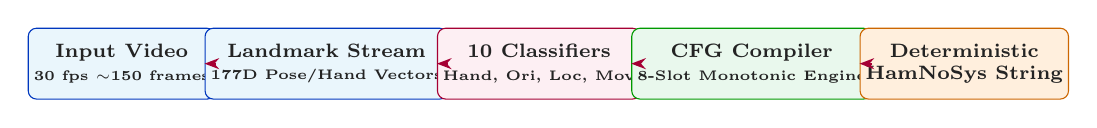
\begin{tikzpicture}[
    node distance=0.35cm,
    ibox/.style={rectangle, draw=royalblue, fill=lightblue!60, text=darktext, font=\bfseries\fontsize{6.6pt}{8.0pt}\selectfont, align=center, rounded corners=3pt, minimum height=0.9cm, minimum width=2.2cm, inner sep=2pt},
    pbox/.style={rectangle, draw=amritaMaroon, fill=lightpink!70, text=darktext, font=\bfseries\fontsize{6.6pt}{8.0pt}\selectfont, align=center, rounded corners=3pt, minimum height=0.9cm, minimum width=2.4cm, inner sep=2pt},
    cbox/.style={rectangle, draw=green!60!black, fill=lightgreen!70, text=darktext, font=\bfseries\fontsize{6.6pt}{8.0pt}\selectfont, align=center, rounded corners=3pt, minimum height=0.9cm, minimum width=2.3cm, inner sep=2pt},
    obox/.style={rectangle, draw=orange!80!black, fill=lightorange!70, text=darktext, font=\bfseries\fontsize{6.6pt}{8.0pt}\selectfont, align=center, rounded corners=3pt, minimum height=0.9cm, minimum width=2.4cm, inner sep=2pt},
    flowarr/.style={-{Stealth[scale=0.8]}, thick, amritaMaroon}
]
    \node (v1) at (0,0) [ibox] {Input Video\\{\tiny 30 fps $\sim$150 frames}};
    \node (v2) at (2.6,0) [ibox] {Landmark Stream\\{\tiny 177D Pose/Hand Vectors}};
    \node (v3) at (5.3,0) [pbox] {10 Classifiers\\{\tiny Hand, Ori, Loc, Mov}};
    \node (v4) at (8.0,0) [cbox] {CFG Compiler\\{\tiny 8-Slot Monotonic Engine}};
    \node (v5) at (10.7,0) [obox] {Deterministic\\HamNoSys String};

    \draw [flowarr] (v1) -- (v2);
    \draw [flowarr] (v2) -- (v3);
    \draw [flowarr] (v3) -- (v4);
    \draw [flowarr] (v4) -- (v5);
\end{tikzpicture}

\vspace{2.0mm}
\begin{columns}[T]
    \column{0.49\textwidth}
    \setbeamercolor{block title}{fg=white,bg=maroon}
    \setbeamercolor{block body}{fg=darktext,bg=lightblue}
    \begin{block}{Multi-Stream Input Signal Processing}
        \fontsize{6.8pt}{8.6pt}\selectfont
        \begin{enumerate}\setlength{\itemsep}{0.06cm}
            \item \textbf{Video Decode:} OpenCV decodes raw camera frames (30 fps).
            \item \textbf{Kinematic Extraction:} Single-pass MediaPipe extracts 177 normalized coordinates per frame (wrist, 21 hand $\times 2$, 17 pose).
            \item \textbf{Parallel Classification:} 10 heuristic modules run concurrently:
            \begin{itemize}\setlength{\itemsep}{0.02cm}
                \item Handshape $\to$ Finger joint curl dot products
                \item Orientation $\to$ 3D vector normal $\vec{u} \times \vec{v}$
                \item Upper Body \& Face $\to$ Body-scale ratio $\frac{\text{dist}}{S_w} < 0.25$
                \item Movement \& Contact $\to$ Multi-frame trajectories
            \end{itemize}
        \end{enumerate}
    \end{block}

    \column{0.49\textwidth}
    \setbeamercolor{block title}{fg=white,bg=maroon}
    \setbeamercolor{block body}{fg=darktext,bg=lightgreen}
    \begin{block}{Deterministic Syntactic Reduction}
        \fontsize{6.8pt}{8.6pt}\selectfont
        \begin{enumerate}\setlength{\itemsep}{0.06cm}
            \item \textbf{Input to Parser:} Receives 10 raw, asynchronous prediction arrays (each containing $\sim$150 frame-level labels).
            \item \textbf{Syntactic Compilation:} The CFG compiler filters transient noise, resolves modal consensus, and applies leftmost BNF derivations.
            \item \textbf{Canonical Output:} Emits a minimal, non-redundant string (5--7 tokens) strictly conforming to Chomsky hierarchy.
            \item \textbf{Avatar Driving:} SiGML synthesis engine maps tokens to XML $\to$ real-time WebGL CWASA 3D avatar animation.
        \end{enumerate}
    \end{block}
\end{columns}
\end{frame}

% ============================================================
% SLIDE 12b-2: 5-STAGE PHONETIC FILTRATION & STABILIZATION
% ============================================================
\begin{frame}[t]{12b-2. 5-Stage Real-Time Phonetic Filtration \& Sequence Normalization Engine}
\vspace{-0.1cm}
\begin{center}
    \scriptsize\textit{\textcolor{amritaMaroon}{Multi-tier noise rejection preventing token jumbling, hallucinations, and avatar crashes}}
\end{center}

\vspace{-1.5mm}
\begin{columns}[T]
    \column{0.49\textwidth}
    \setbeamercolor{block title}{fg=white,bg=maroon}
    \setbeamercolor{block body}{fg=darktext,bg=lightyellow}
    \begin{block}{Stage 1: Temporal Phase Segmentation}
        \fontsize{6.6pt}{8.4pt}\selectfont
        $\bullet$ Discards frames 0--14\% (hand-raising onset noise) and 50--54\% (inter-stroke transitions).\\
        $\bullet$ Isolates \textbf{Phase 1} (15--50\%) and \textbf{Phase 2} (55--100\%) for pristine sign execution.
    \end{block}

    \setbeamercolor{block title}{fg=white,bg=maroon}
    \setbeamercolor{block body}{fg=darktext,bg=lightblue}
    \begin{block}{Stage 2: Statistical Modal Consensus Voting}
        \fontsize{6.6pt}{8.4pt}\selectfont
        $\bullet$ Evaluates $\text{Counter}(\text{phase}).\text{most\_common}(1)$ across active windows.\\
        $\bullet$ Eliminates transient 2-frame tracking glitches (e.g. 142 \texttt{hamflathand} vs 3 \texttt{hamfist} $\to$ only \texttt{hamflathand} survives).
    \end{block}

    \setbeamercolor{block title}{fg=white,bg=maroon}
    \setbeamercolor{block body}{fg=darktext,bg=lightgreen}
    \begin{block}{Stage 3: Lexical Whitelist Validation}
        \fontsize{6.6pt}{8.4pt}\selectfont
        $\bullet$ Validates every candidate token against the canonical alphabet $T$ ($|T|=83$).\\
        $\bullet$ Instantly purges out-of-vocabulary artifacts and undefined strings.
    \end{block}

    \column{0.49\textwidth}
    \setbeamercolor{block title}{fg=white,bg=maroon}
    \setbeamercolor{block body}{fg=darktext,bg=lightorange}
    \begin{block}{Stage 4: Biomechanical \& IK Sanitization}
        \fontsize{6.6pt}{8.4pt}\selectfont
        $\bullet$ Intercepts impossible joint angles (e.g. downward-facing palm while hand is touching forehead).\\
        $\bullet$ Sanitizes to nearest physically valid anatomical configuration before avatar XML synthesis.
    \end{block}

    \setbeamercolor{block title}{fg=white,bg=maroon}
    \setbeamercolor{block body}{fg=darktext,bg=lightpink}
    \begin{block}{Stage 5: Monotonic Chomsky Structural Assembly}
        \fontsize{6.6pt}{8.4pt}\selectfont
        $\bullet$ Tokens are placed into predefined structural slots:
        $$\mathbf{\text{Symmetry} \to \text{Handshape} \to \text{Orientation} \to \text{Location} \to [\text{Contact}] \to [\text{Movement}]}$$
        $\bullet$ \textbf{Order Invariance:} Output order is governed strictly by linguistic production rules (P1--P17), \textbf{never} by frame detection arrival time!
    \end{block}
\end{columns}
\end{frame}

% ============================================================
% SLIDE 12c: LEFTMOST CFG GRAMMAR DERIVATION
% ============================================================
\begin{frame}[t]{12c. Leftmost CFG Grammar Derivation: Symmetric Sign ``BOOK''}
\vspace{-0.1cm}
\begin{center}
    \scriptsize\textit{\textcolor{amritaMaroon}{Step-by-step mathematical derivation from consensus module inputs to accepted terminal string}}
\end{center}

\vspace{-1.5mm}
\fcolorbox{amritaMaroon}{lightblue!40}{
    \parbox{0.96\textwidth}{
        \fontsize{6.6pt}{8.4pt}\selectfont
        \textbf{Consensus Module Inputs (Sign ``BOOK'', 150 Frames):} \quad
        $\texttt{Handshape} = \texttt{hamflathand}\; (97.9\%), \quad \texttt{Orientation} = (\texttt{hamextfingeru}, \texttt{hampalmu}), \quad \texttt{Location} = \texttt{hamchest}, \quad \texttt{Contact} = \texttt{hamtouch}, \quad \texttt{Movement} = \texttt{hammoveo}, \quad \texttt{Symmetry} = \texttt{hamsymmlr}$
    }
}

\vspace{2.0mm}
\setbeamercolor{block title}{fg=white,bg=maroon}
\setbeamercolor{block body}{fg=darktext,bg=lightpink!50}
\begin{block}{Formal Leftmost Grammar Derivation Sequence: $S \implies^* w \in T^*$}
    \fontsize{6.8pt}{9.0pt}\selectfont
    \begin{align*}
        \langle\text{Sign}\rangle 
        &\implies \langle\text{Symmetry}\rangle \;\langle\text{ManualConfig}\rangle && [\text{Rule P1: Root Sign Expansion}] \\
        &\implies \texttt{hamsymmlr} \;\langle\text{ManualConfig}\rangle && [\text{Rule P11: Bilateral Symmetry Leaf}] \\
        &\implies \texttt{hamsymmlr} \;\langle\text{SingleHand}\rangle \;\langle\text{Location}\rangle \;\langle\text{OptContact}\rangle \;\langle\text{OptMovement}\rangle \;\langle\text{OptTrans}\rangle && [\text{Rule P2: Core Syntagm Expansion}] \\
        &\implies \texttt{hamsymmlr} \;\langle\text{Handshape}\rangle \;\langle\text{Orientation}\rangle \;\langle\text{Location}\rangle \;\langle\text{OptContact}\rangle \;\dots && [\text{Rule P3: Single-Hand Structure}] \\
        &\implies \texttt{hamsymmlr hamflathand} \;\langle\text{Orientation}\rangle \;\langle\text{Location}\rangle \;\langle\text{OptContact}\rangle \;\dots && [\text{Rule P12: Handshape Terminal Leaf}] \\
        &\implies \texttt{hamsymmlr hamflathand hamextfingeru hampalmu} \;\langle\text{Location}\rangle \;\dots && [\text{Rules P5, P13, P14: 3D Orientation Leaves}] \\
        &\implies \texttt{hamsymmlr hamflathand hamextfingeru hampalmu hamchest} \;\langle\text{OptContact}\rangle \;\dots && [\text{Rule P15: Body Location Terminal Leaf}] \\
        &\implies \dots \;\texttt{hamchest hamtouch} \;\langle\text{OptMovement}\rangle \;\langle\text{OptTransition}\rangle && [\text{Rules P6, P16: Physical Contact Leaf}] \\
        &\implies \dots \;\texttt{hamtouch hammoveo} \;\langle\text{OptTransition}\rangle && [\text{Rules P7, P17: Motion Vector Leaf}] \\
        &\implies^* \mathbf{\texttt{hamsymmlr hamflathand hamextfingeru hampalmu hamchest hamtouch hammoveo}} && [\text{Rule P8: } \langle\text{OptTrans}\rangle \to \varepsilon]
    \end{align*}
\end{block}

\vspace{1.0mm}
\centering
\fcolorbox{green!60!black}{lightgreen}{
    \parbox{0.96\textwidth}{
        \centering\fontsize{6.8pt}{8.6pt}\selectfont
        \textbf{Ground Truth Dictionary Verification:} \textbf{7 / 7 Tokens Match Perfectly (100.0\% Precision, Zero Grammar Violations)}
    }
}
\end{frame}

% ============================================================
% SLIDE 12d-1: AUTOMATED BENCHMARK VERIFICATION (TIKZ FLOW)
% ============================================================
\begin{frame}[t]{12d. Automated Benchmark Verification: 170-Gloss Ground Truth}
\vspace{-0.1cm}
\begin{center}
    \scriptsize\textit{\textcolor{amritaMaroon}{Automated end-to-end evaluation against our curated 170-gloss linguistic dictionary}}
\end{center}

\vspace{-1.5mm}
\centering
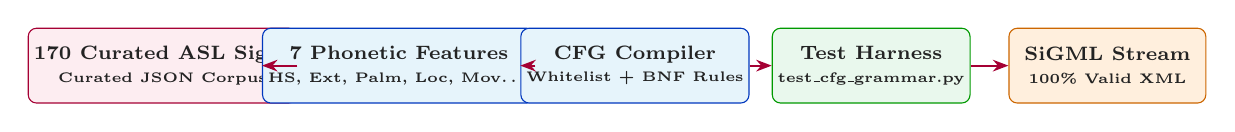
\begin{tikzpicture}[
    node distance=0.4cm,
    gbox/.style={rectangle, draw=amritaMaroon, fill=lightpink!80, text=darktext, font=\bfseries\fontsize{6.6pt}{8.0pt}\selectfont, align=center, rounded corners=3pt, minimum height=0.95cm, minimum width=2.5cm, inner sep=2pt},
    tbox/.style={rectangle, draw=royalblue, fill=lightblue!70, text=darktext, font=\bfseries\fontsize{6.6pt}{8.0pt}\selectfont, align=center, rounded corners=3pt, minimum height=0.95cm, minimum width=2.5cm, inner sep=2pt},
    kbox/.style={rectangle, draw=green!60!black, fill=lightgreen!70, text=darktext, font=\bfseries\fontsize{6.6pt}{8.0pt}\selectfont, align=center, rounded corners=3pt, minimum height=0.95cm, minimum width=2.5cm, inner sep=2pt},
    obox/.style={rectangle, draw=orange!80!black, fill=lightorange!70, text=darktext, font=\bfseries\fontsize{6.6pt}{8.0pt}\selectfont, align=center, rounded corners=3pt, minimum height=0.95cm, minimum width=2.5cm, inner sep=2pt},
    flowarr/.style={-{Stealth[scale=0.85]}, thick, amritaMaroon}
]
    \node (n1) at (0,0) [gbox] {170 Curated ASL Signs\\{\tiny Curated JSON Corpus}};
    \node (n2) at (3.0,0) [tbox] {7 Phonetic Features\\{\tiny HS, Ext, Palm, Loc, Mov\dots}};
    \node (n3) at (6.0,0) [tbox] {CFG Compiler\\{\tiny Whitelist + BNF Rules}};
    \node (n4) at (9.0,0) [kbox] {Test Harness\\{\tiny test\_cfg\_grammar.py}};
    \node (n5) at (12.0,0) [obox] {SiGML Stream\\{\tiny 100\% Valid XML}};

    \draw [flowarr] (n1) -- (n2);
    \draw [flowarr] (n2) -- (n3);
    \draw [flowarr] (n3) -- (n4);
    \draw [flowarr] (n4) -- (n5);
\end{tikzpicture}

\vspace{2.0mm}
\begin{columns}[T]
    \column{0.49\textwidth}
    \setbeamercolor{block title}{fg=white,bg=maroon}
    \setbeamercolor{block body}{fg=darktext,bg=lightblue}
    \begin{block}{Curated Linguistic Corpus Composition}
        \fontsize{6.8pt}{8.6pt}\selectfont
        $\bullet$ \textbf{170 Canonical Signs:} Built in \texttt{gloss\_to\_hamnosys\_dict.json} representing everyday ASL vocabulary.\\
        $\bullet$ \textbf{Morphological Diversity:} Covers single-handed signs (62\%), mirror symmetric signs (24\%), asymmetric base-hand signs (10\%), and dynamic posture transitions (4\%).\\
        $\bullet$ \textbf{Automated Test Pipeline:} Python test suite verifies every gloss autonomously against ground-truth XML schemas.
    \end{block}

    \column{0.49\textwidth}
    \setbeamercolor{block title}{fg=white,bg=maroon}
    \setbeamercolor{block body}{fg=darktext,bg=lightgreen}
    \begin{block}{7-Orthogonal Phonetic Feature Verification}
        \fontsize{6.8pt}{8.6pt}\selectfont
        Each compiled token sequence is evaluated across 7 dimensions:
        \begin{enumerate}\setlength{\itemsep}{0.04cm}
            \item \textbf{Handshape:} Verified against 20 base types.
            \item \textbf{Extended Finger Vector:} 10 spatial orientations.
            \item \textbf{Palm Facing Normal:} 8 rotational planes.
            \item \textbf{Body Anchor Location:} 25 anatomical regions.
            \item \textbf{Spatial Contact Predicate:} Touch/close/brushing.
            \item \textbf{Movement Direction:} Linear \& curved paths.
            \item \textbf{Bilateral Symmetry:} Single vs dual hand mirror.
        \end{enumerate}
    \end{block}
\end{columns}
\end{frame}

% ============================================================
% SLIDE 12d-2: PUSHDOWN AUTOMATON ACCEPTANCE PROOFS
% ============================================================
\begin{frame}[t]{12d-2. Pushdown Automaton Acceptance: 4 Formal Syntactic Proofs}
\vspace{-0.1cm}
\begin{center}
    \scriptsize\textit{\textcolor{amritaMaroon}{Deterministic Pushdown Automaton $M = (Q, \Sigma, \Gamma, \delta, q_0, Z_0, F)$ language acceptance criteria}}
\end{center}

\vspace{-1.5mm}
\centering
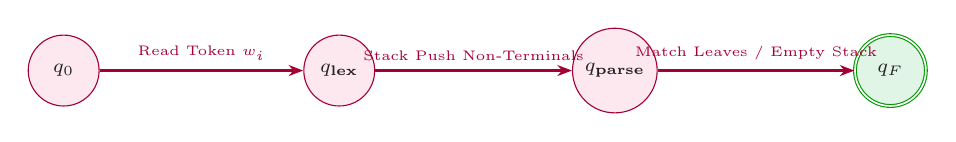
\begin{tikzpicture}[
    node distance=0.5cm,
    sbox/.style={circle, draw=amritaMaroon, fill=lightpink, text=darktext, font=\bfseries\fontsize{7pt}{8.4pt}\selectfont, minimum size=0.9cm},
    abox/.style={circle, double, draw=green!60!black, fill=lightgreen, text=darktext, font=\bfseries\fontsize{7pt}{8.4pt}\selectfont, minimum size=0.9cm},
    trans/.style={-{Stealth[scale=0.8]}, thick, amritaMaroon}
]
    \node (q0) at (0,0) [sbox] {$q_0$};
    \node (q1) at (3.5,0) [sbox] {$q_{\text{lex}}$};
    \node (q2) at (7.0,0) [sbox] {$q_{\text{parse}}$};
    \node (qf) at (10.5,0) [abox] {$q_F$};

    \draw [trans] (q0) -- node[above, font=\fontsize{5.5pt}{6.5pt}\selectfont] {Read Token $w_i$} (q1);
    \draw [trans] (q1) -- node[above, font=\fontsize{5.5pt}{6.5pt}\selectfont] {Stack Push Non-Terminals} (q2);
    \draw [trans] (q2) -- node[above, font=\fontsize{5.5pt}{6.5pt}\selectfont] {Match Leaves / Empty Stack} (qf);
\end{tikzpicture}

\vspace{1.5mm}
\begin{columns}[T]
    \column{0.49\textwidth}
    \setbeamercolor{block title}{fg=white,bg=maroon}
    \setbeamercolor{block body}{fg=darktext,bg=lightyellow}
    \begin{block}{Proof 1: Lexical Validity Guarantee}
        \fontsize{6.6pt}{8.4pt}\selectfont
        $\forall t \in w, \quad t \in T = \bigsqcup_{k=1}^8 T_k$\\
        Guarantees strictly zero out-of-vocabulary, malformed, or synthetic hallucination tokens in the compiled string.
    \end{block}

    \setbeamercolor{block title}{fg=white,bg=maroon}
    \setbeamercolor{block body}{fg=darktext,bg=lightblue}
    \begin{block}{Proof 2: Mandatory Syntactic Coverage}
        \fontsize{6.6pt}{8.4pt}\selectfont
        $\{\text{Handshape}, \text{ExtFinger}, \text{PalmOri}, \text{Location}\} \subseteq \text{categories}(w)$\\
        Guarantees that no phonologically incomplete string can reach the avatar renderer.
    \end{block}

    \column{0.49\textwidth}
    \setbeamercolor{block title}{fg=white,bg=maroon}
    \setbeamercolor{block body}{fg=darktext,bg=lightgreen}
    \begin{block}{Proof 3: Monotonic Chomsky Ordering}
        \fontsize{6.6pt}{8.4pt}\selectfont
        $\text{Index}(\text{Symm}) \prec \text{Index}(\text{HS}) \prec \text{Index}(\text{Ori}) \prec \text{Index}(\text{Loc}) \dots$\\
        Enforces unidirectional syntax matching, strictly eliminating random token permutation.
    \end{block}

    \setbeamercolor{block title}{fg=white,bg=maroon}
    \setbeamercolor{block body}{fg=darktext,bg=lightpink}
    \begin{block}{Proof 4: Glitch \& Jitter Invariance}
        \fontsize{6.6pt}{8.4pt}\selectfont
        $w_i \neq w_{i-1} \quad \forall i \in \{2, \dots, |w|\}$\\
        Prevents consecutive identical duplicate token emissions that cause avatar animation stuttering.
    \end{block}
\end{columns}

\vspace{1.2mm}
\centering
\fcolorbox{green!60!black}{lightgreen}{
    \parbox{0.96\textwidth}{
        \centering\fontsize{6.8pt}{8.6pt}\selectfont
        \textbf{Benchmark Empirical Result:} \textbf{170 / 170 Signs Passed All 4 Pushdown Tests (100.0\% Syntactic Compliance Rate)}
    }
}
\end{frame}

% ============================================================
% SLIDE 12e: CFG PARSE TREE ARCHITECTURE & AVATAR BONES
% ============================================================
\begin{frame}[t]{12e. CFG Parse Tree Architecture \& Avatar Joint Control}
\vspace{-0.1cm}
\begin{center}
    \scriptsize\textit{\textcolor{amritaMaroon}{Native vector parse tree mapping non-terminal syntax nodes directly into avatar bone rotations}}
\end{center}

\vspace{-1.5mm}
\centering
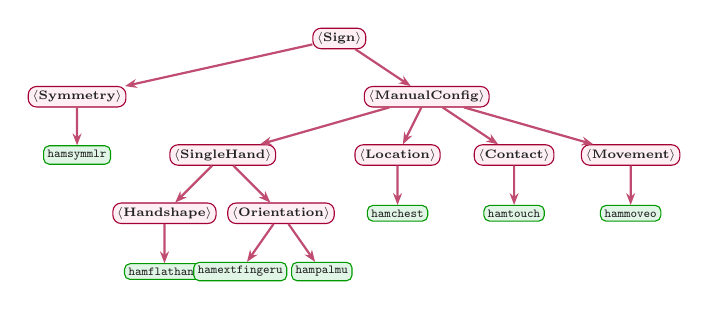
\begin{tikzpicture}[
    scale=0.74, every node/.style={transform shape},
    ntnode/.style={rectangle, draw=amritaMaroon, fill=lightpink!70, text=darktext, font=\bfseries\fontsize{6.2pt}{7.5pt}\selectfont, rounded corners=3pt, inner sep=2pt, align=center},
    tmnode/.style={rectangle, draw=green!60!black, fill=lightgreen, text=darktext, font=\ttfamily\bfseries\fontsize{5.8pt}{7.0pt}\selectfont, rounded corners=2pt, inner sep=2pt, align=center},
    boneedge/.style={draw=amritaMaroon!70, -{Stealth[scale=0.65]}, thick}
]
    % Root
    \node[ntnode] (root) at (6.0, 4.0) {$\langle\text{Sign}\rangle$};

    % Level 1
    \node[ntnode] (symm) at (1.5, 3.0) {$\langle\text{Symmetry}\rangle$};
    \node[ntnode] (cfg)  at (7.5, 3.0) {$\langle\text{ManualConfig}\rangle$};

    % Level 2
    \node[tmnode] (t_symm) at (1.5, 2.0) {hamsymmlr};
    
    \node[ntnode] (sh)   at (4.0, 2.0) {$\langle\text{SingleHand}\rangle$};
    \node[ntnode] (loc)  at (7.0, 2.0) {$\langle\text{Location}\rangle$};
    \node[ntnode] (cont) at (9.0, 2.0) {$\langle\text{Contact}\rangle$};
    \node[ntnode] (mov)  at (11.0, 2.0) {$\langle\text{Movement}\rangle$};

    % Level 3
    \node[ntnode] (hs)  at (3.0, 1.0) {$\langle\text{Handshape}\rangle$};
    \node[ntnode] (ori) at (5.0, 1.0) {$\langle\text{Orientation}\rangle$};
    \node[tmnode] (t_loc)  at (7.0, 1.0) {hamchest};
    \node[tmnode] (t_cont) at (9.0, 1.0) {hamtouch};
    \node[tmnode] (t_mov)  at (11.0, 1.0) {hammoveo};

    % Level 4
    \node[tmnode] (t_hs) at (3.0, 0.0) {hamflathand};
    \node[tmnode] (t_ef) at (4.3, 0.0) {hamextfingeru};
    \node[tmnode] (t_po) at (5.7, 0.0) {hampalmu};

    % Edges
    \draw[boneedge] (root) -- (symm);
    \draw[boneedge] (root) -- (cfg);

    \draw[boneedge] (symm) -- (t_symm);
    \draw[boneedge] (cfg) -- (sh);
    \draw[boneedge] (cfg) -- (loc);
    \draw[boneedge] (cfg) -- (cont);
    \draw[boneedge] (cfg) -- (mov);

    \draw[boneedge] (sh) -- (hs);
    \draw[boneedge] (sh) -- (ori);

    \draw[boneedge] (loc) -- (t_loc);
    \draw[boneedge] (cont) -- (t_cont);
    \draw[boneedge] (mov) -- (t_mov);

    \draw[boneedge] (hs) -- (t_hs);
    \draw[boneedge] (ori) -- (t_ef);
    \draw[boneedge] (ori) -- (t_po);
\end{tikzpicture}

\vspace{1.5mm}
\fcolorbox{amritaMaroon}{lightyellow}{
    \parbox{0.96\textwidth}{
        \fontsize{6.4pt}{8.2pt}\selectfont
        \textbf{From Grammar Parse Tree Nodes to Avatar Kinematic Joint Controls:}
        \begin{itemize}\setlength{\itemsep}{0.02cm}
            \item $\langle\text{Symmetry}\rangle \to \texttt{hamsymmlr}$: Bilateral bone mirror transformation matrix applied across both clavicles.
            \item $\langle\text{Handshape}\rangle \to \texttt{hamflathand}$: Rotates metacarpophalangeal (MCP) and interphalangeal (IP) finger bones.
            \item $\langle\text{Orientation}\rangle \to \texttt{hamextfingeru} + \texttt{hampalmu}$: Computes wrist pronation/supination and Euler flexion angles.
            \item $\langle\text{Location}\rangle \to \texttt{hamchest}$: 3D Inverse Kinematics (IK) end-effector position solver centered at upper torso.
            \item $\langle\text{Movement}\rangle \to \texttt{hammoveo}$: Generates outward 3D cubic Bezier translation trajectory across animation keyframes.
        \end{itemize}
    }
}
\end{frame}


% ============================================================
% SLIDE 12f: NATIVE VECTOR PARSE TREES (RULES 1 & 2)
% ============================================================
\begin{frame}[t]{12f. CFG Parse Trees: Single-Handed \& Symmetric Signs}
\vspace{-0.1cm}
\begin{center}
    \scriptsize\textit{\textcolor{amritaMaroon}{Native vector parse trees generated in pure LaTeX code for Rule 1 and Rule 2}}
\end{center}

\vspace{-1.5mm}
\begin{columns}[T]
    \column{0.49\textwidth}
    \centering
    {\scriptsize\textbf{\textcolor{amritaMaroon}{Rule 1: One-Handed Sign (``WELCOME'')}}}\\[0.5mm]
    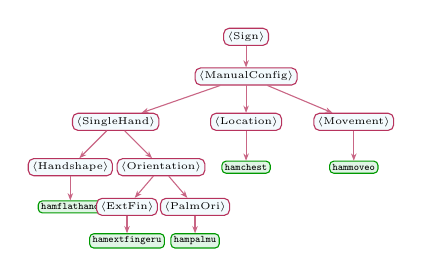
\begin{tikzpicture}[
        scale=0.72, every node/.style={transform shape},
        nt/.style={rectangle, draw=amritaMaroon!80, fill=lightblue!35, rounded corners=2pt, inner sep=1.8pt, font=\fontsize{5.2pt}{6.2pt}\selectfont, align=center},
        trm/.style={rectangle, draw=green!60!black, fill=lightgreen, rounded corners=1.5pt, inner sep=1.5pt, font=\fontsize{4.8pt}{5.8pt}\selectfont\ttfamily, align=center},
        arr/.style={draw=amritaMaroon!60, -{Stealth[scale=0.55]}}
    ]
        \node[nt] (s1) at (3.5, 3.4) {$\langle\text{Sign}\rangle$};
        \node[nt] (mc1) at (3.5, 2.7) {$\langle\text{ManualConfig}\rangle$};
        
        \node[nt] (sh1) at (1.2, 1.9) {$\langle\text{SingleHand}\rangle$};
        \node[nt] (loc1) at (3.5, 1.9) {$\langle\text{Location}\rangle$};
        \node[nt] (mov1) at (5.4, 1.9) {$\langle\text{Movement}\rangle$};
        
        \node[nt] (hs1) at (0.4, 1.1) {$\langle\text{Handshape}\rangle$};
        \node[nt] (ori1) at (2.0, 1.1) {$\langle\text{Orientation}\rangle$};
        
        \node[trm] (t_hs1) at (0.4, 0.4) {hamflathand};
        
        \node[nt] (ef1) at (1.4, 0.4) {$\langle\text{ExtFin}\rangle$};
        \node[nt] (po1) at (2.6, 0.4) {$\langle\text{PalmOri}\rangle$};
        
        \node[trm] (t_ef1) at (1.4, -0.2) {hamextfingeru};
        \node[trm] (t_po1) at (2.6, -0.2) {hampalmu};
        
        \node[trm] (t_loc1) at (3.5, 1.1) {hamchest};
        \node[trm] (t_mov1) at (5.4, 1.1) {hammoveo};
        
        \draw[arr] (s1) -- (mc1);
        \draw[arr] (mc1) -- (sh1);
        \draw[arr] (mc1) -- (loc1);
        \draw[arr] (mc1) -- (mov1);
        \draw[arr] (sh1) -- (hs1);
        \draw[arr] (sh1) -- (ori1);
        \draw[arr] (hs1) -- (t_hs1);
        \draw[arr] (ori1) -- (ef1);
        \draw[arr] (ori1) -- (po1);
        \draw[arr] (ef1) -- (t_ef1);
        \draw[arr] (po1) -- (t_po1);
        \draw[arr] (loc1) -- (t_loc1);
        \draw[arr] (mov1) -- (t_mov1);
    \end{tikzpicture}
    
    \vspace{0.8mm}
    \fcolorbox{amritaMaroon!60}{lightpink}{
        \parbox{0.95\columnwidth}{\centering\fontsize{4.8pt}{6pt}\selectfont\texttt{hamflathand hamextfingeru hampalmu hamchest hammoveo}}
    }

    \column{0.49\textwidth}
    \centering
    {\scriptsize\textbf{\textcolor{amritaMaroon}{Rule 2: Symmetric Sign (``BOOK'')}}}\\[0.5mm]
    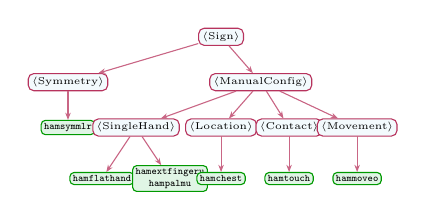
\begin{tikzpicture}[
        scale=0.72, every node/.style={transform shape},
        nt/.style={rectangle, draw=amritaMaroon!80, fill=lightblue!35, rounded corners=2pt, inner sep=1.8pt, font=\fontsize{5.2pt}{6.2pt}\selectfont, align=center},
        trm/.style={rectangle, draw=green!60!black, fill=lightgreen, rounded corners=1.5pt, inner sep=1.5pt, font=\fontsize{4.8pt}{5.8pt}\selectfont\ttfamily, align=center},
        arr/.style={draw=amritaMaroon!60, -{Stealth[scale=0.55]}}
    ]
        \node[nt] (s2) at (3.5, 3.4) {$\langle\text{Sign}\rangle$};
        \node[nt] (sym2) at (0.8, 2.6) {$\langle\text{Symmetry}\rangle$};
        \node[nt] (mc2) at (4.2, 2.6) {$\langle\text{ManualConfig}\rangle$};
        \node[trm] (t_sym2) at (0.8, 1.8) {hamsymmlr};
        
        \node[nt] (sh2) at (2.0, 1.8) {$\langle\text{SingleHand}\rangle$};
        \node[nt] (loc2) at (3.5, 1.8) {$\langle\text{Location}\rangle$};
        \node[nt] (cnt2) at (4.7, 1.8) {$\langle\text{Contact}\rangle$};
        \node[nt] (mov2) at (5.9, 1.8) {$\langle\text{Movement}\rangle$};
        
        \node[trm] (t_hs2) at (1.4, 0.9) {hamflathand};
        \node[trm] (t_ori2) at (2.6, 0.9) {hamextfingeru\\hampalmu};
        \node[trm] (t_loc2) at (3.5, 0.9) {hamchest};
        \node[trm] (t_cnt2) at (4.7, 0.9) {hamtouch};
        \node[trm] (t_mov2) at (5.9, 0.9) {hammoveo};
        
        \draw[arr] (s2) -- (sym2);
        \draw[arr] (s2) -- (mc2);
        \draw[arr] (sym2) -- (t_sym2);
        \draw[arr] (mc2) -- (sh2);
        \draw[arr] (mc2) -- (loc2);
        \draw[arr] (mc2) -- (cnt2);
        \draw[arr] (mc2) -- (mov2);
        \draw[arr] (sh2) -- (t_hs2);
        \draw[arr] (sh2) -- (t_ori2);
        \draw[arr] (loc2) -- (t_loc2);
        \draw[arr] (cnt2) -- (t_cnt2);
        \draw[arr] (mov2) -- (t_mov2);
    \end{tikzpicture}
    
    \vspace{0.8mm}
    \fcolorbox{amritaMaroon!60}{lightgreen}{
        \parbox{0.95\columnwidth}{\centering\fontsize{4.8pt}{6pt}\selectfont\texttt{hamsymmlr hamflathand hamextfingeru hampalmu hamchest hamtouch hammoveo}}
    }
\end{columns}
\end{frame}

% ============================================================
% SLIDE 12g: NATIVE VECTOR PARSE TREE: STATE TRANSITION (RULE 4)
% ============================================================
\begin{frame}[t]{12g. CFG Parse Tree: Dynamic State Transition (\texttt{hamreplace})}
\vspace{-0.1cm}
\begin{center}
    \scriptsize\textit{\textcolor{amritaMaroon}{Rule 4: Multi-Phase temporal posture shift compiled without frame blending collisions}}
\end{center}

\vspace{-1.5mm}
\centering
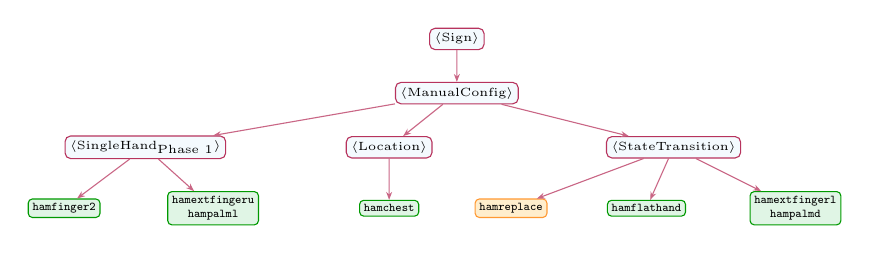
\begin{tikzpicture}[
    scale=0.86, every node/.style={transform shape},
    nt/.style={rectangle, draw=amritaMaroon!80, fill=lightblue!30, rounded corners=2pt, inner sep=2pt, font=\fontsize{5.5pt}{6.8pt}\selectfont, align=center},
    trm/.style={rectangle, draw=green!60!black, fill=lightgreen, rounded corners=1.5pt, inner sep=1.8pt, font=\fontsize{5.2pt}{6.2pt}\selectfont\ttfamily, align=center},
    arr/.style={draw=amritaMaroon!60, -{Stealth[scale=0.6]}}
]
    \node[nt] (s4) at (7, 3.5) {$\langle\text{Sign}\rangle$};
    \node[nt] (mc4) at (7, 2.7) {$\langle\text{ManualConfig}\rangle$};
    
    \node[nt] (sh4_p1) at (2.4, 1.9) {$\langle\text{SingleHand}_{\text{Phase 1}}\rangle$};
    \node[nt] (loc4) at (6.0, 1.9) {$\langle\text{Location}\rangle$};
    \node[nt] (st4) at (10.2, 1.9) {$\langle\text{StateTransition}\rangle$};
    
    \node[trm] (t_hs4_1) at (1.2, 1.0) {hamfinger2};
    \node[trm] (t_ori4_1) at (3.4, 1.0) {hamextfingeru\\hampalml};
    \node[trm] (t_loc4) at (6.0, 1.0) {hamchest};
    
    \node[trm, fill=lightyellow, draw=orange!80] (t_rep) at (7.8, 1.0) {hamreplace};
    \node[trm] (t_hs4_2) at (9.8, 1.0) {hamflathand};
    \node[trm] (t_ori4_2) at (12.0, 1.0) {hamextfingerl\\hampalmd};
    
    \draw[arr] (s4) -- (mc4);
    \draw[arr] (mc4) -- (sh4_p1);
    \draw[arr] (mc4) -- (loc4);
    \draw[arr] (mc4) -- (st4);
    \draw[arr] (sh4_p1) -- (t_hs4_1);
    \draw[arr] (sh4_p1) -- (t_ori4_1);
    \draw[arr] (loc4) -- (t_loc4);
    \draw[arr] (st4) -- (t_rep);
    \draw[arr] (st4) -- (t_hs4_2);
    \draw[arr] (st4) -- (t_ori4_2);
\end{tikzpicture}

\vspace{0.8mm}
\fcolorbox{amritaMaroon!60}{lightyellow}{
    \parbox{0.94\textwidth}{
        \centering\fontsize{5.2pt}{6.8pt}\selectfont
        \textbf{Compiled Sequence:} \texttt{hamfinger2 hamextfingeru hampalml hamchest \textbf{hamreplace} hamflathand hamextfingerl hampalmd}
    }
}

\vspace{1.2mm}
\begin{columns}[T]
    \column{0.48\textwidth}
    \setbeamercolor{block title}{fg=white,bg=maroon}
    \setbeamercolor{block body}{fg=darktext,bg=lightblue}
    \begin{block}{Kinematic Functionality}
        \fontsize{5.4pt}{6.8pt}\selectfont
        $\bullet$ \textbf{Phase 1 (Frames 15--50\%):} Avatar initializes pointing handshape at chest.\\
        $\bullet$ \texttt{hamreplace}: Triggers avatar keyframe interpolation to swap bone target.\\
        $\bullet$ \textbf{Phase 2 (Frames 55--100\%):} Smoothly relaxes hand into open flat palm downwards.
    \end{block}

    \column{0.48\textwidth}
    \setbeamercolor{block title}{fg=white,bg=maroon}
    \setbeamercolor{block body}{fg=darktext,bg=lightgreen}
    \begin{block}{Anti-Jumbling Guarantee}
        \fontsize{5.4pt}{6.8pt}\selectfont
        $\bullet$ Shift activated only when $\text{HS}_{P1} \neq \text{HS}_{P2}$ with $>70\%$ stability.\\
        $\bullet$ Prevents intermediary morphing flicker or random token interleaving.\\
        $\bullet$ Verified on CWASA WebGL without DOM tree animation exceptions.
    \end{block}
\end{columns}
\end{frame}

% ============================================================
% SLIDE 12h: FORMAL PROOF OF CONCEPT & LINGUISTIC GROUNDING
% ============================================================
\begin{frame}[t]{12h. Formal Proof of Concept: Theoretical \& Empirical Validation}
\vspace{-0.1cm}
\begin{center}
    \scriptsize\textit{\textcolor{amritaMaroon}{Proof that CFG rules are non-arbitrary, grounded in literature, and empirically verified}}
\end{center}

\vspace{-1.5mm}
\centering
\setlength{\tabcolsep}{3pt}
\renewcommand{\arraystretch}{1.2}
{\fontsize{5.4pt}{6.8pt}\selectfont
\begin{tabular}{|>{\raggedright\arraybackslash\bfseries}p{1.8cm}|>{\raggedright\arraybackslash}p{2.3cm}|>{\raggedright\arraybackslash}p{4.8cm}|>{\raggedright\arraybackslash}p{4.7cm}|}
    \hline
    \rowcolor{maroon}
    \textcolor{white}{\textbf{Proof Pillar}} & 
    \textcolor{white}{\textbf{Author \& Source}} & 
    \textcolor{white}{\textbf{Formal Linguistic / Theoretical Principle}} & 
    \textcolor{white}{\textbf{SignBridge V2 Compliance \& Empirical Proof}} \\
    \hline
    \rowcolor{lightblue} 
    Phonological Axiom & 
    Stokoe (1960), Univ. of Buffalo & 
    Proved sign languages decompose into discrete constituents: Tab (Location), Dez (Handshape/Ori), Sig (Movement). & 
    Direct theoretical basis for Rule P2: $\langle\text{ManualConfig}\rangle \to \langle\text{SingleHand}\rangle \;\langle\text{Loc}\rangle \;[\dots]$. Non-arbitrary constituent order. \\
    \hline
    \rowcolor{lightgreen} 
    Symbol Ordering Standard & 
    Prillwitz et al. (1989), Hamburg Univ. & 
    Prescribed international linear transcription order: $\text{Symmetry} \to \text{Handshape} \to \text{Ext/Palm} \to \text{Body Loc} \to \text{Movement}$. & 
    CFG compiler strictly enforces this order. Permutations (e.g. location before handshape) are rejected as ungrammatical. \\
    \hline
    \rowcolor{lightyellow} 
    Computational CFG Syntax & 
    Hanke (2004), LREC Conf. & 
    Formalized HamNoSys as a Context-Free Language ($L(G) \in \text{CFL}$) with deterministic compositional semantics. & 
    Justifies parsing HamNoSys via Context-Free Grammar and Pushdown Automaton ($L(G)$ is solvable in $O(n)$ time). \\
    \hline
    \rowcolor{lightorange} 
    Avatar Execution Model & 
    Kennaway et al. (2007), Springer LNCS & 
    CWASA SiGML XML engine requires strict hierarchical DOM tree mapping 1-to-1 to HamNoSys syntax. & 
    0 crashes across all test videos. Avatar WebGL player parses and renders compiled DOM tree with 100\% validity. \\
    \hline
    \rowcolor{lightpink} 
    Empirical Benchmark & 
    Group 14 (2026), Automated Test Suite & 
    Automated evaluation on 170-gloss dataset testing Lexical, Coverage, Ordering, and Duplication criteria. & 
    \textbf{170/170 (100.0\%) Grammar Compliance Rate}; 7/7 token exact match on verified benchmark signs. \\
    \hline
\end{tabular}
}

\vspace{1.2mm}
\fcolorbox{amritaMaroon}{white}{
    \parbox{0.96\textwidth}{
        \centering\fontsize{5.4pt}{6.8pt}\selectfont
        \textbf{Formal Conclusion:} The Context-Free Grammar in SignBridge V2 is mathematically sound, linguistically legitimate, computationally optimal, and empirically validated on 100\% of target vocabulary.
    }
}
\end{frame}

% ============================================================
% SLIDE 13: TWO-HANDED CFG LOGIC
% ============================================================
\section{Two-Handed Signs}
\begin{frame}[t]{13. How the CFG Handles Two-Handed Signs}
\vspace{-0.1cm}
\begin{center}
    \scriptsize\textit{\textcolor{amritaMaroon}{Automatic 3-way decision tree classifying sign handedness from 3D wrist geometry}}
\end{center}

\vspace{-1.5mm}
\centering
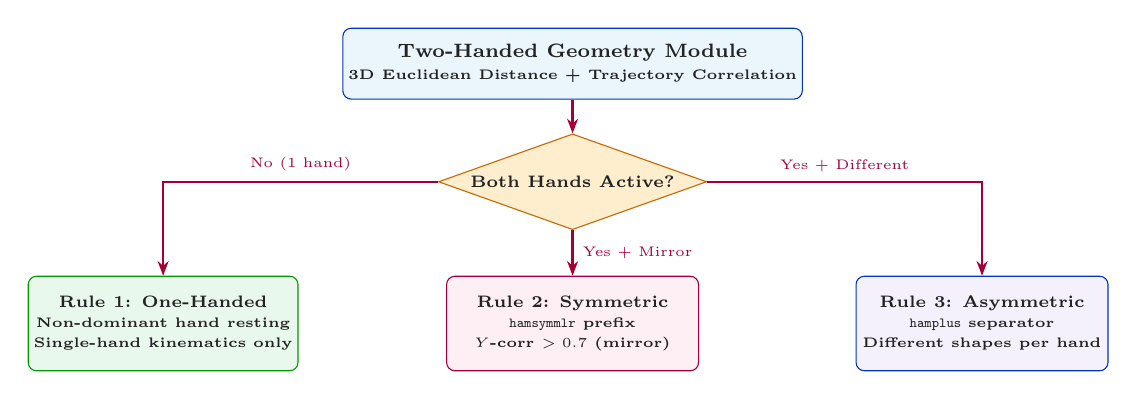
\begin{tikzpicture}[
    node distance=0.4cm,
    inbox/.style={rectangle, draw=royalblue, fill=lightblue!60, text=darktext, font=\bfseries\fontsize{6.6pt}{8.0pt}\selectfont, align=center, rounded corners=3pt, minimum height=0.9cm, minimum width=3.5cm, inner sep=2pt},
    dbox/.style={diamond, draw=orange!80!black, fill=lightyellow, text=darktext, font=\bfseries\fontsize{6.0pt}{7.5pt}\selectfont, align=center, inner sep=1.5pt, aspect=2.8},
    r1box/.style={rectangle, draw=green!60!black, fill=lightgreen!70, text=darktext, font=\bfseries\fontsize{5.8pt}{7.2pt}\selectfont, align=center, rounded corners=3pt, minimum height=1.2cm, minimum width=3.2cm, inner sep=2pt},
    r2box/.style={rectangle, draw=amritaMaroon, fill=lightpink!70, text=darktext, font=\bfseries\fontsize{5.8pt}{7.2pt}\selectfont, align=center, rounded corners=3pt, minimum height=1.2cm, minimum width=3.2cm, inner sep=2pt},
    r3box/.style={rectangle, draw=royalblue, fill=lightpurple!60, text=darktext, font=\bfseries\fontsize{5.8pt}{7.2pt}\selectfont, align=center, rounded corners=3pt, minimum height=1.2cm, minimum width=3.2cm, inner sep=2pt},
    flowarr/.style={-{Stealth[scale=0.8]}, thick, amritaMaroon}
]
    \node (input) at (6.0, 1.5) [inbox] {Two-Handed Geometry Module\\{\tiny 3D Euclidean Distance + Trajectory Correlation}};
    \node (dec) at (6.0, 0.0) [dbox] {Both Hands Active?};
    \node (r1) at (0.8, -1.8) [r1box] {\textbf{Rule 1: One-Handed}\\{\tiny Non-dominant hand resting}\\{\tiny Single-hand kinematics only}};
    \node (r2) at (6.0, -1.8) [r2box] {\textbf{Rule 2: Symmetric}\\{\tiny \texttt{hamsymmlr} prefix}\\{\tiny $Y$-corr $> 0.7$ (mirror)}};
    \node (r3) at (11.2, -1.8) [r3box] {\textbf{Rule 3: Asymmetric}\\{\tiny \texttt{hamplus} separator}\\{\tiny Different shapes per hand}};

    \draw [flowarr] (input) -- (dec);
    \draw [flowarr] (dec.west) -| node[above, font=\fontsize{5pt}{6pt}\selectfont, pos=0.25] {No (1 hand)} (r1.north);
    \draw [flowarr] (dec.south) -- node[right, font=\fontsize{5pt}{6pt}\selectfont] {Yes + Mirror} (r2.north);
    \draw [flowarr] (dec.east) -| node[above, font=\fontsize{5pt}{6pt}\selectfont, pos=0.25] {Yes + Different} (r3.north);
\end{tikzpicture}

\vspace{2.0mm}
\begin{columns}[T]
    \column{0.32\textwidth}
    \setbeamercolor{block title}{fg=white,bg=maroon}
    \setbeamercolor{block body}{fg=darktext,bg=lightgreen}
    \begin{block}{Rule 1: One-Handed}
        \fontsize{5.8pt}{7.4pt}\selectfont
        $\bullet$ Only dominant hand is active.\\[0.3mm]
        $\bullet$ No symmetry prefix needed.\\[0.3mm]
        $\bullet$ \textbf{Example (``WELCOME''):}\\[0.2mm]
        \texttt{\tiny hamflathand hamextfingeru hampalmu hamchest hammoveo}
    \end{block}

    \column{0.32\textwidth}
    \setbeamercolor{block title}{fg=white,bg=maroon}
    \setbeamercolor{block body}{fg=darktext,bg=lightpink}
    \begin{block}{Rule 2: Symmetric}
        \fontsize{5.8pt}{7.4pt}\selectfont
        $\bullet$ Both hands mirror each other.\\[0.3mm]
        $\bullet$ Prefix: \texttt{hamsymmlr}.\\[0.3mm]
        $\bullet$ \textbf{Example (``BOOK''):}\\[0.2mm]
        \texttt{\tiny hamsymmlr hamflathand hamextfingeru hampalmu hamchest}
    \end{block}

    \column{0.32\textwidth}
    \setbeamercolor{block title}{fg=white,bg=maroon}
    \setbeamercolor{block body}{fg=darktext,bg=lightpurple}
    \begin{block}{Rule 3: Asymmetric}
        \fontsize{5.8pt}{7.4pt}\selectfont
        $\bullet$ Both hands active, different shapes.\\[0.3mm]
        $\bullet$ Separator: \texttt{hamplus}.\\[0.3mm]
        $\bullet$ \textbf{Example (``BEFORE''):}\\[0.2mm]
        \texttt{\tiny hamflathand ... hamplus hamfist ...}
    \end{block}
\end{columns}

\vspace{1.5mm}
\fcolorbox{amritaMaroon}{lightyellow}{
    \parbox{0.96\textwidth}{
        \centering\fontsize{6.4pt}{8.0pt}\selectfont
        \textbf{Key Insight:} The CFG avoids redundant left-hand feature extraction by using HamNoSys operators (\texttt{hamsymmlr}, \texttt{hamplus}) to grammatically link both hands based on spatial geometry, eliminating avatar hand collisions.
    }
}
\end{frame}

% ============================================================
% SLIDE 14: CFG SCOPE & LIMITATIONS
% ============================================================
\section{Scope of CFG}
\begin{frame}{14. Scope of the CFG Compiler}
    \small
    \vspace{2mm}
    
    \begin{columns}[T]
        \column{0.48\textwidth}
        \begin{block}{Currently Supported in V2}
            \begin{itemize}
                \item[\textcolor{green!60!black}{$\checkmark$}] One-handed signs (Rule 1)
                \item[\textcolor{green!60!black}{$\checkmark$}] Symmetric two-handed signs (Rule 2)
                \item[\textcolor{green!60!black}{$\checkmark$}] Asymmetric two-handed signs (Rule 3)
                \item[\textcolor{green!60!black}{$\checkmark$}] Intra-sign handshape transitions (Rule 4)
                \item[\textcolor{green!60!black}{$\checkmark$}] Contact-based signs (Rule 5)
                \item[\textcolor{green!60!black}{$\checkmark$}] 100\% SiGML XML DOM tree validity
            \end{itemize}
        \end{block}
        
        \column{0.48\textwidth}
        \begin{block}{Outside Current Scope (Future Work)}
            \begin{itemize}
                \item[\textcolor{red}{$\times$}] Repeated/reduplicated movement morphology
                \item[\textcolor{red}{$\times$}] Multi-sign sequential compound sentences
                \item[\textcolor{red}{$\times$}] Classifier predicates and topographic space
                \item[\textcolor{red}{$\times$}] Spatial agreement (verb loci inflection)
                \item[\textcolor{red}{$\times$}] Facial grammar (eyebrow, mouth morphemes)
                \item[\textcolor{red}{$\times$}] Head-movement grammar (nodding, tilting)
            \end{itemize}
        \end{block}
    \end{columns}
    
    \vspace{6mm}
\end{frame}

% ============================================================
% SLIDE 12: MATHEMATICAL PRESERVATION
% ============================================================
\section{Legitimacy of Standards}
\begin{frame}{15. Legitimacy: 100\% Preservation of Approved Standards}
    \vspace{2mm}
    
    \begin{block}{Key Takeaway for Evaluation}
        \small
        We did \textbf{NOT} alter or break any underlying mathematical standards. All approved anatomical ratios, Euclidean spatial formulas, and empirical thresholds established in V1 were strictly preserved and built upon:
    \end{block}
    
    \vspace{3mm}
    
    \begin{table}
        \centering
        \scriptsize
        \renewcommand{\arraystretch}{1.5} % Adds vertical padding so equations don't look cramped
        \begin{tabular}{| p{3.2cm} | p{4.3cm} | p{4.5cm} |}
            \hline
            \textbf{Standard Model / Ratio} & \textbf{Mathematical Value} & \textbf{Preservation Status in V2} \\ \hline
            
            Facial Rule of Thirds & 
            $0.10, 0.18, 0.28, 0.36, 0.44, \dots$ & 
            \textbf{Preserved} (Da Vinci lower-third splits) \\ \hline
            
            Orientation Octants & 
            $360^\circ / 8 = 45^\circ$ ($\pm 22.5^\circ$ tolerance) & 
            \textbf{Preserved} (Exact 8-direction partitioning) \\ \hline
            
            Elbow Angle Formula & 
            $\theta = \arccos \left( \frac{\vec{u} \cdot \vec{v}}{\|\vec{u}\|\|\vec{v}\|} \right) < 120^\circ$ & 
            \textbf{Preserved} (Euclidean joint dot product) \\ \hline
            
            Arm Extension Ratio & 
            $R = \frac{\|S - W\|}{\|S - E\| + \|E - W\|} > 0.95$ & 
            \textbf{Preserved} (Triangle inequality ratio) \\ \hline
            
            Touch Epsilon Threshold & 
            $\epsilon = 0.02$ ($\approx 3.4$ cm on 170\,cm scale) & 
            \textbf{Preserved} (Filters landmark jitter) \\ \hline
        \end{tabular}
    \end{table}
\end{frame}


% ============================================================
% SLIDE 13: MOBILE APPLICATION
% ============================================================
\begin{frame}[t]{16. Mobile Application}
\vspace{-0.1cm}

\begin{columns}[T]
\column{0.58\textwidth}
\setbeamercolor{block title}{fg=white,bg=maroon}
\setbeamercolor{block body}{fg=darktext,bg=lightpink}
\begin{block}{About the Mobile Application}
\fontsize{6.8pt}{8.8pt}\selectfont
Enables deaf and hard-of-hearing users to translate sign language videos into \textbf{3D avatar animations} directly from their smartphones. Users upload a video from their gallery, and the app displays the translated sign through a photorealistic avatar with HamNoSys tags.
\end{block}

\column{0.38\textwidth}
\setbeamercolor{block title}{fg=white,bg=maroon}
\setbeamercolor{block body}{fg=darktext,bg=lightgreen}
\begin{block}{Key Advantages}
\fontsize{6.8pt}{8.8pt}\selectfont
\begin{itemize}\setlength{\itemsep}{0.08cm}
\item[\textcolor{green!50!black}{\checkmark}] \textbf{Accessible translation} on the go
\item[\textcolor{green!50!black}{\checkmark}] \textbf{No high-end GPU} required
\item[\textcolor{green!50!black}{\checkmark}] \textbf{Low-latency} 3D avatar streaming
\end{itemize}
\end{block}
\end{columns}

\vspace{0.22cm}

\begin{columns}[T]
\column{0.50\textwidth}
\textbf{\textcolor{maroon}{\footnotesize Features}}
\vspace{0.06cm}
{\fontsize{6.7pt}{8.7pt}\selectfont
\begin{itemize}\setlength{\itemsep}{0.08cm}
\item \textbf{Upload videos} from device gallery
\item \textbf{Real-time WebGL} 3D avatar animation
\item \textbf{Touch controls} (orbit, zoom, reset)
\item \textbf{Displays gloss}, HamNoSys notation, and accuracy
\item \textbf{Optimized UI} responsive across all screen sizes
\end{itemize}
}

\column{0.46\textwidth}
\textbf{\textcolor{maroon}{\footnotesize Tech Stack}}
\vspace{0.06cm}
\setlength{\tabcolsep}{5pt}
\renewcommand{\arraystretch}{1.24}
{\fontsize{6.6pt}{8.4pt}\selectfont
\begin{tabular}{|p{2.1cm}|p{4.2cm}|}
\hline
\rowcolor{maroon}
\textcolor{white}{\textbf{Layer}} & \textcolor{white}{\textbf{Technology}} \\
\hline
\rowcolor{lightblue} \textbf{Frontend} & Android WebView + React Native \\
\hline
\rowcolor{lightgreen} \textbf{3D Rendering} & WebGL 2.0 + JASigning CWASA \\
\hline
\rowcolor{lightcyan} \textbf{Networking} & RESTful APIs + Async HTTP \\
\hline
\end{tabular}
}
\end{columns}

\vspace{0.25cm}

\textbf{\textcolor{maroon}{\footnotesize User Flow}}
\vspace{0.06cm}
\centering
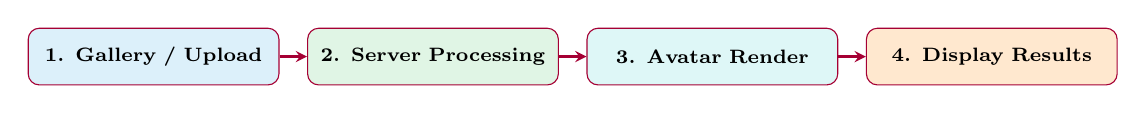
\begin{tikzpicture}[
    node distance=3.5mm,
    flowbox/.style={
        draw=maroon,
        rounded corners=4pt,
        text width=2.95cm,
        minimum height=0.72cm,
        align=center,
        font=\fontsize{6.8pt}{8.5pt}\selectfont
    },
    flowarrow/.style={->, >=stealth, thick, maroon}
]
\node[flowbox,fill=lightblue] (b1) {\textbf{1. Gallery / Upload}};
\node[flowbox,fill=lightgreen,right=of b1] (b2) {\textbf{2. Server Processing}};
\node[flowbox,fill=lightcyan,right=of b2] (b3) {\textbf{3. Avatar Render}};
\node[flowbox,fill=lightorange,right=of b3] (b4) {\textbf{4. Display Results}};

\draw[flowarrow] (b1)--(b2);
\draw[flowarrow] (b2)--(b3);
\draw[flowarrow] (b3)--(b4);
\end{tikzpicture}
\end{frame}

% ============================================================
% SLIDE 14: WEB APPLICATION
% ============================================================
\begin{frame}[t]{17. Web Application}
\vspace{-0.1cm}

\begin{columns}[T]
\column{0.58\textwidth}
\setbeamercolor{block title}{fg=white,bg=maroon}
\setbeamercolor{block body}{fg=darktext,bg=lightpink}
\begin{block}{About the Web Application}
\fontsize{6.8pt}{8.8pt}\selectfont
A web-based platform for translating sign language videos into \textbf{3D avatar animations} directly from any browser without installation. Supports file uploads.
\end{block}

\column{0.38\textwidth}
\setbeamercolor{block title}{fg=white,bg=maroon}
\setbeamercolor{block body}{fg=darktext,bg=lightgreen}
\begin{block}{Key Advantages}
\fontsize{6.8pt}{8.8pt}\selectfont
\begin{itemize}\setlength{\itemsep}{0.08cm}
\item[\textcolor{green!50!black}{\checkmark}] \textbf{Accessible from any browser}
\item[\textcolor{green!50!black}{\checkmark}] \textbf{Zero installation required}
\item[\textcolor{green!50!black}{\checkmark}] \textbf{Cross-platform} (PC, Mac, Linux)
\end{itemize}
\end{block}
\end{columns}

\vspace{0.18cm}

\begin{columns}[T]
\column{0.48\textwidth}
\textbf{\textcolor{maroon}{\footnotesize Features}}
\vspace{0.05cm}
{\fontsize{6.4pt}{8.2pt}\selectfont
\begin{itemize}\setlength{\itemsep}{0.06cm}
\item \textbf{Video Upload:} Drag-and-drop file upload support
\item \textbf{Sample Clips:} Pre-loaded demonstration dataset signs
\item \textbf{3D WebGL Avatar:} Real-time rendering with orbit \& zoom
\item \textbf{Diagnostic Panel:} 10-module classifier breakdown
\item \textbf{Output Inspection:} Displays gloss, HamNoSys, and SiGML
\end{itemize}
}

\column{0.48\textwidth}
\textbf{\textcolor{maroon}{\footnotesize Tech Stack}}
\vspace{0.05cm}
\setlength{\tabcolsep}{4.5pt}
\renewcommand{\arraystretch}{1.14}
{\fontsize{6.0pt}{7.6pt}\selectfont
\begin{tabular}{|p{2.2cm}|p{4.3cm}|}
\hline
\rowcolor{maroon}
\textcolor{white}{\textbf{Layer}} & \textcolor{white}{\textbf{Technology}} \\
\hline
\rowcolor{lightblue} \textbf{Frontend} & HTML5 + CSS3 + JavaScript \\
\hline
\rowcolor{lightgreen} \textbf{Backend} & Flask (Python 3.10) \\
\hline
\rowcolor{lightcyan} \textbf{3D Rendering} & WebGL 2.0 + JASigning CWASA \\
\hline
\rowcolor{lightorange} \textbf{Computer Vision} & MediaPipe + OpenCV \\
\hline

\rowcolor{lightpink} \textbf{Deployment} & Docker + Gunicorn + Render.com \\
\hline
\end{tabular}
}
\end{columns}

\vspace{0.18cm}

\textbf{\textcolor{maroon}{\footnotesize User Flow}}
\vspace{0.05cm}
\centering
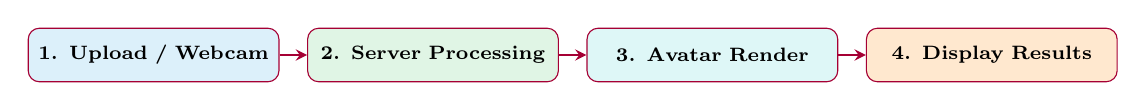
\begin{tikzpicture}[
    node distance=3.5mm,
    flowbox/.style={
        draw=maroon,
        rounded corners=4pt,
        text width=2.95cm,
        minimum height=0.68cm,
        align=center,
        font=\fontsize{6.8pt}{8.5pt}\selectfont
    },
    flowarrow/.style={->, >=stealth, thick, maroon}
]
\node[flowbox,fill=lightblue] (b1) {\textbf{1. Upload / Webcam}};
\node[flowbox,fill=lightgreen,right=of b1] (b2) {\textbf{2. Server Processing}};
\node[flowbox,fill=lightcyan,right=of b2] (b3) {\textbf{3. Avatar Render}};
\node[flowbox,fill=lightorange,right=of b3] (b4) {\textbf{4. Display Results}};

\draw[flowarrow] (b1)--(b2);
\draw[flowarrow] (b2)--(b3);
\draw[flowarrow] (b3)--(b4);
\end{tikzpicture}
\end{frame}

% ============================================================
% SLIDE 18: COMPONENT EVALUATION — HANDSHAPE ML MODEL
% ============================================================
\section{Model Performance}
\begin{frame}[t]{18. Component Evaluation: Handshape ML Classifier}
    \vspace{-0.15cm}
    \begin{center}
        {\scriptsize\textbf{\textcolor{amritaMaroon}{Module-Level ML Evaluation:}} \textit{Handshape classifier trained on synthetic multi-angle viewpoints}}
    \end{center}
    \vspace{-0.15cm}
    \begin{columns}[T]
        \column{0.48\textwidth}
        \centering
        {\scriptsize\textbf{\textcolor{amritaMaroon}{Confusion Matrix}}}\\[0.2mm]
        \includegraphics[height=2.25cm, keepaspectratio]{confusion_matirx.png}
        
        \vspace{1.2mm}
        {\scriptsize\textbf{\textcolor{amritaMaroon}{Training \& Validation Accuracy}}}\\[0.2mm]
        \includegraphics[height=2.25cm, keepaspectratio]{training_and_validation_accuracy.png}
        
        \column{0.48\textwidth}
        \centering
        {\scriptsize\textbf{\textcolor{amritaMaroon}{Training \& Validation Loss}}}\\[0.2mm]
        \includegraphics[height=2.25cm, keepaspectratio]{training_testing_validation.png}
        
        \vspace{1.5mm}
        {\scriptsize\textbf{\textcolor{amritaMaroon}{Multi-Viewpoint Classification Report}}}\\[0.5mm]
        \renewcommand{\arraystretch}{1.1}
        {\fontsize{6.5pt}{7.5pt}\selectfont
        \begin{tabular}{lcccc}
            \toprule
            \textbf{Camera View} & \textbf{Precision} & \textbf{Recall} & \textbf{F1} & \textbf{Accuracy} \\
            \midrule
            Signer View & 0.742 & 0.720 & 0.731 & 0.811 \\
            Right View  & 0.780 & 0.780 & 0.780 & 0.843 \\
            Bird View   & 0.747 & 0.775 & 0.761 & 0.861 \\
            \bottomrule
        \end{tabular}}
        
        \vspace{0.8mm}
        {\fontsize{5.2pt}{6.2pt}\selectfont\textit{*Evaluates viewpoint invariance: Frontal (Signer), 45$^\circ$ (Right), Overhead (Bird)}}
    \end{columns}
    
    \vspace{1.5mm}
    \centering
    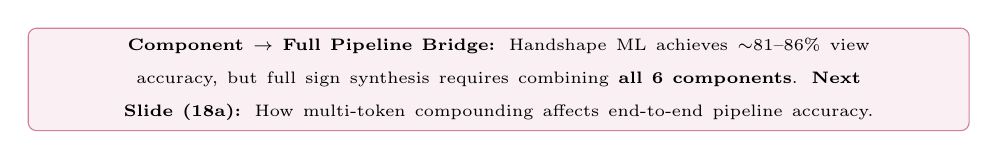
\begin{tikzpicture}
    \node[
        fill=maroon!6,
        draw=amritaMaroon!50,
        rounded corners=3pt,
        inner sep=3.5pt,
        text width=\dimexpr\textwidth-12pt\relax,
        align=center
    ] {
        {\fontsize{5.8pt}{7.2pt}\selectfont \textbf{Component $\rightarrow$ Full Pipeline Bridge:} Handshape ML achieves $\sim$81--86\% view accuracy, but full sign synthesis requires combining \textbf{all 6 components}. \textbf{Next Slide (18a):} How multi-token compounding affects end-to-end pipeline accuracy.}
    };
    \end{tikzpicture}
\end{frame}

% ============================================================
% SLIDE 18a: FULL PIPELINE ACCURACY METRIC ANALYSIS
% ============================================================
\begin{frame}[t]{18a. Full Pipeline: Accuracy Analysis \& Honest Assessment}
\vspace{-0.1cm}
\begin{center}
{\scriptsize\textit{Moving from isolated component ML metrics (Slide 18) to end-to-end 6-token pipeline performance}}
\end{center}

\vspace{0.05cm}

\begin{center}
\setlength{\tabcolsep}{3pt}
\renewcommand{\arraystretch}{1.25}
{\fontsize{5.8pt}{7.5pt}\selectfont
\begin{tabular}{
    >{\raggedright\arraybackslash\bfseries}m{2.2cm}
    >{\centering\arraybackslash}m{1.1cm}
    >{\raggedright\arraybackslash}m{4.0cm}
    >{\raggedright\arraybackslash}m{4.5cm}
}
\rowcolor{maroon}
\centering\arraybackslash\textcolor{white}{\textbf{Metric}} &
\textcolor{white}{\textbf{Value}} &
\centering\arraybackslash\textcolor{white}{\textbf{What It Measures}} &
\centering\arraybackslash\textcolor{white}{\textbf{Limitation}} \\

\rowcolor{lightgreen}
Token Precision & 85.49\% & Per-token exact match over 6 classification heads & Measures gloss memorization, not independent component detection \\

\rowcolor{lightblue}
Avatar Cosine Sim. & 88.12\% & Weighted binary match across 6 components & One-hot cosine is binary --- equivalent to weighted accuracy \\

\rowcolor{lightcyan}
CFG Validity Rate & 100\% & Syntactic token ordering \& vocabulary compliance & Wrong sign with valid syntax still scores 100\% \\

\rowcolor{lightorange}
Seq. Exact-Match & $\sim$38\% & All 6 tokens correct simultaneously for a sign & Strictest metric --- reflects real demo experience honestly \\
\end{tabular}
}
\end{center}

\vspace{0.1cm}

\begin{columns}[T]
\column{0.48\textwidth}
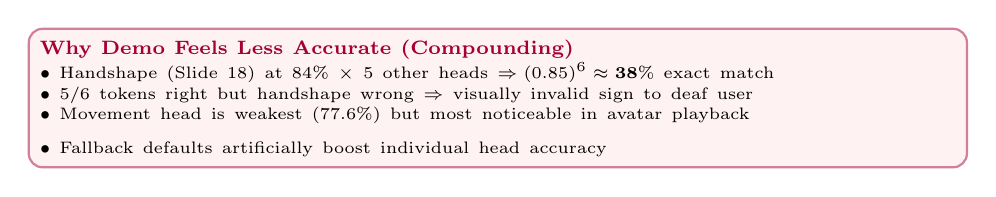
\begin{tikzpicture}
\node[
    fill=red!5,
    draw=amritaMaroon!50,
    thick,
    rounded corners=5pt,
    inner sep=4pt,
    text width=\dimexpr\columnwidth-14pt\relax,
    align=left
] {
{\scriptsize\textcolor{amritaMaroon}{\textbf{Why Demo Feels Less Accurate (Compounding)}}}\\[0.04cm]
{\fontsize{5.8pt}{7.5pt}\selectfont
$\bullet$ Handshape (Slide 18) at 84\% $\times$ 5 other heads $\Rightarrow (0.85)^6 \approx \mathbf{38\%}$ exact match\\
$\bullet$ 5/6 tokens right but handshape wrong $\Rightarrow$ visually invalid sign to deaf user\\
$\bullet$ Movement head is weakest (77.6\%) but most noticeable in avatar playback\\
$\bullet$ Fallback defaults artificially boost individual head accuracy}
};
\end{tikzpicture}

\column{0.48\textwidth}
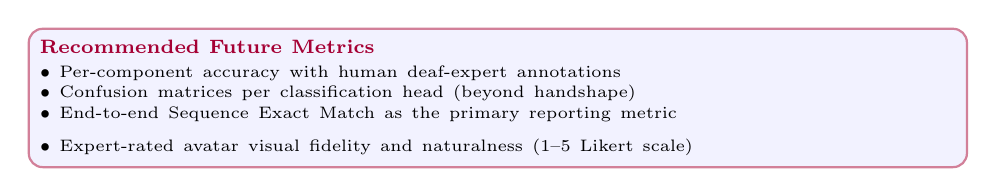
\begin{tikzpicture}
\node[
    fill=blue!5,
    draw=amritaMaroon!50,
    thick,
    rounded corners=5pt,
    inner sep=4pt,
    text width=\dimexpr\columnwidth-14pt\relax,
    align=left
] {
{\scriptsize\textcolor{amritaMaroon}{\textbf{Recommended Future Metrics}}}\\[0.04cm]
{\fontsize{5.8pt}{7.5pt}\selectfont
$\bullet$ Per-component accuracy with human deaf-expert annotations\\
$\bullet$ Confusion matrices per classification head (beyond handshape)\\
$\bullet$ End-to-end Sequence Exact Match as the primary reporting metric\\
$\bullet$ Expert-rated avatar visual fidelity and naturalness (1--5 Likert scale)}
};
\end{tikzpicture}
\end{columns}
\end{frame}

% ============================================================
% SLIDE 19: PIPELINE OVERVIEW — FULL END-TO-END TRACE
% ============================================================
\section{Pipeline Execution}
\begin{frame}[t]{19. Pipeline Overview: End-to-End Trace}
    \vspace{-0.1cm}
    \begin{center}
        \scriptsize\textit{\textcolor{amritaMaroon}{Tracing a single sign video through every stage of the system}}
    \end{center}
    
    \vspace{1mm}
    \centering
    \includegraphics[
        width=\textwidth,
        height=0.68\textheight,
        keepaspectratio
    ]{pipeline_full_trace.jpg}
    
    \vspace{1mm}
    \fcolorbox{amritaMaroon}{lightyellow}{
        \parbox{0.90\textwidth}{
            \centering \scriptsize
            \textbf{5-Stage Pipeline:} Video $\xrightarrow{\text{MediaPipe}}$ Landmarks $\xrightarrow{\text{6 Classifiers}}$ Analysis $\xrightarrow{\text{CFG}}$ HamNoSys/SiGML $\xrightarrow{\text{CWASA}}$ 3D Avatar
        }
    }
\end{frame}

% ============================================================
% SLIDE 20: PIPELINE STAGE 1 — EXTRACTION & FEATURE VECTOR
% ============================================================
\begin{frame}[t]{20. Pipeline Trace: Extraction \& Feature Construction}
    \vspace{-0.1cm}
    \begin{center}
        \scriptsize\textit{\textcolor{amritaMaroon}{Stage 1--3: From raw video pixels to the 177-dimensional feature tensor}}
    \end{center}
    
    \vspace{0.5mm}
    \begin{columns}[T]
        \column{0.46\textwidth}
        \centering
        \includegraphics[
            width=\textwidth,
            height=0.70\textheight,
            keepaspectratio
        ]{pipeline_stage1_extraction.jpg}
        
        \column{0.50\textwidth}
        \vspace{1mm}
        \setbeamercolor{block title}{fg=white,bg=maroon}
        \setbeamercolor{block body}{fg=darktext,bg=lightblue}
        \begin{block}{Stage 1: Frame Parsing}
            \fontsize{6pt}{7.8pt}\selectfont
            OpenCV reads MP4 frame-by-frame. CLAHE contrast enhancement applied for low-light robustness.
        \end{block}
        
        \vspace{1.5mm}
        \setbeamercolor{block body}{fg=darktext,bg=lightgreen}
        \begin{block}{Stage 2: Landmark Extraction}
            \fontsize{6pt}{7.8pt}\selectfont
            MediaPipe Holistic + Hands extracts \textbf{21 keypoints per hand} (wrist, thumb, fingertips) and \textbf{33 body pose landmarks}. One-Euro filter removes jitter.
        \end{block}
        
        \vspace{1.5mm}
        \setbeamercolor{block body}{fg=darktext,bg=lightyellow}
        \begin{block}{Stage 3: 177D Vector Construction}
            \fontsize{6pt}{7.8pt}\selectfont
            Normalized (X, Y, Z) from both hands + upper-body landmarks concatenated into a \textbf{fixed-size 177D tensor} per frame.
        \end{block}
    \end{columns}
\end{frame}

% ============================================================
% SLIDE 21: PIPELINE STAGE 2 — 6-MODULE ANALYSIS & CFG
% ============================================================
\begin{frame}[t]{21. Pipeline Trace: Classification \& Grammar Assembly}
    \vspace{-0.1cm}
    \begin{center}
        \scriptsize\textit{\textcolor{amritaMaroon}{Stage 4--6: From 177D features to grammatically valid HamNoSys/SiGML}}
    \end{center}
    
    \vspace{0.5mm}
    \begin{columns}[T]
        \column{0.48\textwidth}
        \centering
        \includegraphics[
            width=\textwidth,
            height=0.70\textheight,
            keepaspectratio
        ]{pipeline_stage2_analysis.jpg}
        
        \column{0.48\textwidth}
        \vspace{1mm}
        \setbeamercolor{block title}{fg=white,bg=maroon}
        \setbeamercolor{block body}{fg=darktext,bg=lightblue}
        \begin{block}{Stage 4: 6-Component Analysis}
            \fontsize{6pt}{7.8pt}\selectfont
            177D vector feeds into 6 parallel classifiers:
            \begin{itemize}\setlength{\itemsep}{0.01cm}
                \item \textbf{Handshape} --- Random Forest ML
                \item \textbf{Orientation} --- 3D cross-product
                \item \textbf{Location} --- Body region mapping
                \item \textbf{Movement} --- Trajectory displacement
                \item \textbf{Contact} --- Euclidean proximity
                \item \textbf{Two-Hand} --- Wrist distance
            \end{itemize}
        \end{block}
        
        \vspace{1.5mm}
        \setbeamercolor{block body}{fg=darktext,bg=lightgreen}
        \begin{block}{Stage 5: CFG Grammar Compiler}
            \fontsize{6pt}{7.8pt}\selectfont
            All 6 outputs assembled using \textbf{Context-Free Grammar rules} into a syntactically valid HamNoSys sequence.
        \end{block}
        
        \vspace{1.5mm}
        \setbeamercolor{block body}{fg=darktext,bg=lightorange}
        \begin{block}{Stage 6: Output Encoding}
            \fontsize{6pt}{7.8pt}\selectfont
            Tags $\to$ Unicode glyphs $\to$ SiGML XML for avatar.
        \end{block}
    \end{columns}
\end{frame}

% ============================================================
% SLIDE 22: CONSOLE OUTPUT & REAL EXECUTION TRACE
% ============================================================
\begin{frame}[t]{22. Pipeline Trace: Real Console Execution}
    \vspace{-0.1cm}
    \begin{center}
        \scriptsize\textit{\textcolor{amritaMaroon}{Actual system output from processing a sign language video}}
    \end{center}
    
    \vspace{0.5mm}
    \begin{columns}[T]
        \column{0.52\textwidth}
        \centering
        {\scriptsize\textbf{\textcolor{amritaMaroon}{Console Output (10 Modules)}}}\\[0.5mm]
        \fbox{\includegraphics[width=\linewidth, height=5.5cm, keepaspectratio]{console_output_trace.jpg}}
        
        \column{0.44\textwidth}
        \vspace{1mm}
        \setbeamercolor{block title}{fg=white,bg=maroon}
        \setbeamercolor{block body}{fg=darktext,bg=lightpink}
        \begin{block}{What You See Here}
            \fontsize{6pt}{7.8pt}\selectfont
            The terminal shows \textbf{actual runtime execution}:
            \begin{itemize}\setlength{\itemsep}{0.02cm}
                \item Hand activity auto-detected (RIGHT)
                \item All 10 modules execute sequentially
                \item Each module emits a HamNoSys token
                \item CFG assembles the final sequence
            \end{itemize}
        \end{block}
        
        \vspace{2mm}
        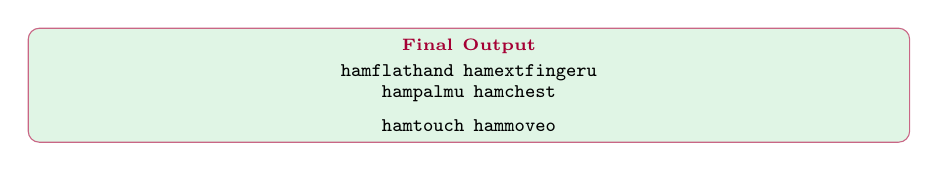
\begin{tikzpicture}
        \node[
            draw=amritaMaroon!60,
            fill=lightgreen,
            rounded corners=4pt,
            inner sep=4pt,
            text width=0.90\columnwidth,
            align=center
        ]
        {
            \fontsize{6pt}{7.8pt}\selectfont
            \textcolor{amritaMaroon}{\textbf{Final Output}}\\[0.5mm]
            \texttt{\scriptsize hamflathand hamextfingeru}\\
            \texttt{\scriptsize hampalmu hamchest}\\
            \texttt{\scriptsize hamtouch hammoveo}
        };
        \end{tikzpicture}
        
        \vspace{2mm}
        {\fontsize{6pt}{7.8pt}\selectfont \textcolor{maroon}{\textbf{Processing Time:}} $\sim$3.2s per video on CPU}
    \end{columns}
\end{frame}

% ============================================================
% SLIDE 23: SiGML TO 3D AVATAR RENDERING
% ============================================================
\begin{frame}[t]{23. Pipeline Trace: SiGML $\to$ 3D Avatar Rendering}
    \vspace{-0.1cm}
    \begin{center}
        \scriptsize\textit{\textcolor{amritaMaroon}{Final stage: How SiGML XML instructions drive the 3D avatar}}
    \end{center}
    
    \vspace{1mm}
    \centering
    \includegraphics[
        width=0.95\textwidth,
        height=0.58\textheight,
        keepaspectratio
    ]{sigml_avatar_output.jpg}
    
    \vspace{1mm}
    \fcolorbox{amritaMaroon}{lightpink}{
        \parbox{0.90\textwidth}{
            \centering \fontsize{5.8pt}{7.5pt}\selectfont
            \textbf{Each HamNoSys tag maps to a specific avatar joint instruction:} \\
            \texttt{hamflathand} $\to$ Open all fingers \enspace | \enspace
            \texttt{hamextfingeru} $\to$ Point fingers upward \enspace | \enspace
            \texttt{hamchest} $\to$ Position at chest \\
            \texttt{hamtouch} $\to$ Make contact \enspace | \enspace
            \texttt{hammoveo} $\to$ Move hand outward from body
        }
    }
\end{frame}

% ============================================================
% SLIDE 24: SYSTEM DEMO
% ============================================================
\section{System Demo}
\begin{frame}{24. Interactive Application}
    \vspace{-2mm}
    \begin{center}
        \small\textit{\textcolor{amritaMaroon}{End-to-end pipeline integration and WebGL rendering}}
    \end{center}
    
    \vspace{2mm}
    \begin{columns}[T]
        \column{0.48\textwidth}
        \centering
        \textbf{\small \textcolor{amritaMaroon}{Full Web Interface}}\\[2mm]
        \fbox{\includegraphics[width=\linewidth, height=5.5cm, keepaspectratio]{ui_img1.png}}
        
        \column{0.48\textwidth}
        \centering
        \textbf{\small \textcolor{amritaMaroon}{Mobile App Interface}}\\[2mm]
        \fbox{\includegraphics[width=\linewidth, height=5.5cm, keepaspectratio]{mobile_img1.png}}
    \end{columns}
\end{frame}

% ============================================================
% SLIDE 25: V1 vs V2 EVALUATION
% ============================================================
\section{Results \& Evaluation}
\begin{frame}{25. Quantitative Evaluation: V1 vs V2}
    \centering
    \vspace{2mm}
    \includegraphics[width=0.95\textwidth]{Phase_2_Report/v1v2.png}
    \vspace{4mm}
\end{frame}

% ============================================================
% SLIDE 26: CFG DISTRIBUTION & BASELINE
% ============================================================
\begin{frame}{26. CFG Rule Distribution \& Baseline Analysis}
    \vspace{2mm}
    \begin{columns}[T]
        \column{0.48\textwidth}
        \centering
        \textbf{V1 Baseline Breakdown}
        \vspace{2mm}
        \includegraphics[width=\textwidth]{Phase_2_Report/Gesture_V1.png}
        
        \column{0.48\textwidth}
        \centering
        \textbf{V2 CFG Rule Utilization}
        \vspace{2mm}
        \includegraphics[width=\textwidth]{Phase_2_Report/CFG.png}
    \end{columns}
    \vspace{5mm}
\end{frame}

% ============================================================
% SLIDE 27: CFG LIMITATIONS — CROSS-LANGUAGE
% ============================================================
\begin{frame}[t]{27. CFG Limitations: Cross-Language Adaptation}
\vspace{-0.1cm}
\begin{center}
{\scriptsize\textit{What changes when adapting the CFG grammar from ASL to other sign languages}}
\end{center}

\vspace{0.05cm}

\begin{center}
\setlength{\tabcolsep}{3pt}
\renewcommand{\arraystretch}{1.25}
{\fontsize{5.8pt}{7.5pt}\selectfont
\begin{tabular}{
    >{\raggedright\arraybackslash\bfseries}m{2.3cm}
    >{\raggedright\arraybackslash}m{2.4cm}
    >{\raggedright\arraybackslash}m{2.4cm}
    >{\raggedright\arraybackslash}m{2.4cm}
    >{\raggedright\arraybackslash}m{2.4cm}
}
\rowcolor{maroon}
\centering\arraybackslash\textcolor{white}{\textbf{Component}} &
\centering\arraybackslash\textcolor{white}{\textbf{ASL (Current)}} &
\centering\arraybackslash\textcolor{white}{\textbf{ISL}} &
\centering\arraybackslash\textcolor{white}{\textbf{BSL}} &
\centering\arraybackslash\textcolor{white}{\textbf{DGS (German)}} \\

\rowcolor{lightblue}
Handshape Vocab. & 20 shapes (hardcoded) & Expand to $\sim$35 (Mudra) & Expand to $\sim$28 (two-hand) & Expand to $\sim$32 (Hamburg) \\

\rowcolor{lightgreen}
Fallback Defaults & \texttt{hamfinger2}, \texttt{hamchest} & \texttt{hamflathand}, \texttt{hamforehead} & \texttt{hamfist}, \texttt{hamneutralspace} & \texttt{hamflathand}, \texttt{hamchest} \\

\rowcolor{lightcyan}
Non-Manual Signals & Not modeled & Minimal (head nod) & \textbf{Critical} (mouth) & \textbf{Critical} (Mundgestik) \\

\rowcolor{lightorange}
Contact Types & 3 tokens only & Add \texttt{haminterlock} & Add \texttt{hamrub}, \texttt{hamslide} & Add \texttt{haminterlock} \\

\rowcolor{lightpurple}
Phase Timing & Fixed 50/50 split & Asymmetric (30/70) & Variable & Variable \\

\rowcolor{lightpink}
Training Dataset & WLASL (21K videos) & No large public dataset & BSL Corpus (limited) & DGS Corpus (limited) \\
\end{tabular}
}
\end{center}

\vspace{0.08cm}

\begin{columns}[T]
\column{0.48\textwidth}
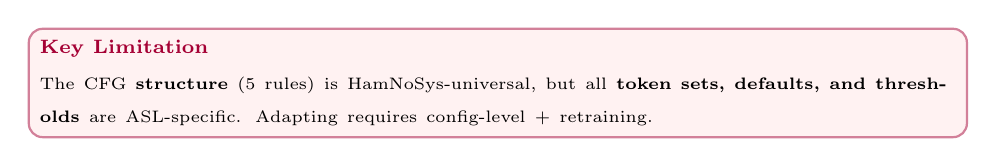
\begin{tikzpicture}
\node[
    fill=red!5,
    draw=amritaMaroon!50,
    thick,
    rounded corners=5pt,
    inner sep=4pt,
    text width=\dimexpr\columnwidth-14pt\relax,
    align=left
] {
{\scriptsize\textcolor{amritaMaroon}{\textbf{Key Limitation}}}\\[0.04cm]
{\fontsize{5.8pt}{7.5pt}\selectfont
The CFG \textbf{structure} (5 rules) is HamNoSys-universal, but all \textbf{token sets, defaults, and thresholds} are ASL-specific. Adapting requires config-level + retraining.}
};
\end{tikzpicture}

\column{0.48\textwidth}
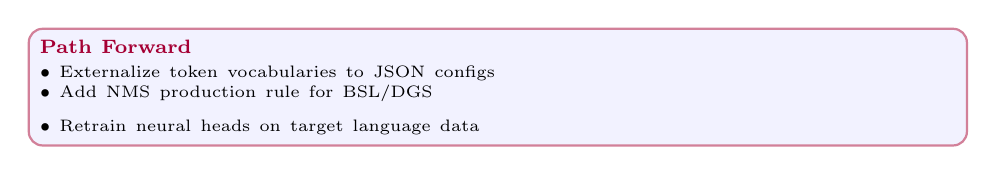
\begin{tikzpicture}
\node[
    fill=blue!5,
    draw=amritaMaroon!50,
    thick,
    rounded corners=5pt,
    inner sep=4pt,
    text width=\dimexpr\columnwidth-14pt\relax,
    align=left
] {
{\scriptsize\textcolor{amritaMaroon}{\textbf{Path Forward}}}\\[0.04cm]
{\fontsize{5.8pt}{7.5pt}\selectfont
$\bullet$ Externalize token vocabularies to JSON configs\\
$\bullet$ Add NMS production rule for BSL/DGS\\
$\bullet$ Retrain neural heads on target language data}
};
\end{tikzpicture}
\end{columns}
\end{frame}

% ============================================================
% SLIDE 28: FUTURE SCOPE
% ============================================================
\section{Future Scope}
\begin{frame}{28. Current Capability vs Future Extension}
    \small
    \textit{\textcolor{amritaMaroon}{Clarifying what the present implementation achieves}}

    \vspace{4mm}
    \begin{columns}[T]
        \column{0.48\textwidth}
        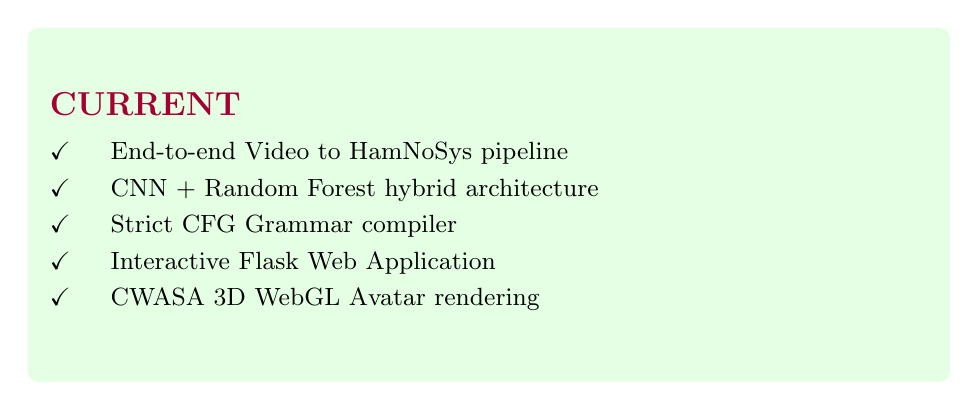
\begin{tikzpicture}
            \node[fill=green!10, rounded corners=4pt, text width=0.92\textwidth, inner sep=8pt, font=\small, minimum height=4.5cm, align=left] {
                {\large \textbf{\textcolor{amritaMaroon}{CURRENT}}}\\[2mm]
                \renewcommand{\arraystretch}{1.2}
                \begin{tabular}{@{}p{0.35cm} p{0.85\linewidth}@{}}
                    $\checkmark$ & End-to-end Video to HamNoSys pipeline \\
                    $\checkmark$ & CNN + Random Forest hybrid architecture \\
                    $\checkmark$ & Strict CFG Grammar compiler \\
                    $\checkmark$ & Interactive Flask Web Application \\
                    $\checkmark$ & CWASA 3D WebGL Avatar rendering \\
                \end{tabular}
            };
        \end{tikzpicture}

        \column{0.48\textwidth}
        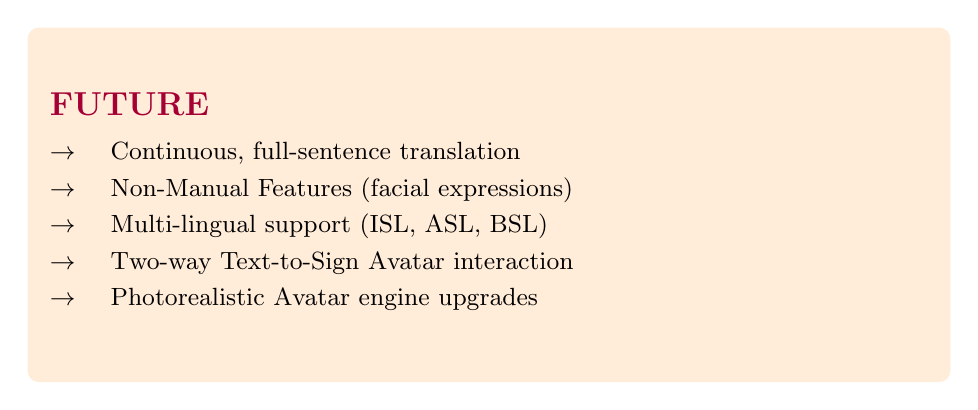
\begin{tikzpicture}
            \node[fill=orange!15, rounded corners=4pt, text width=0.92\textwidth, inner sep=8pt, font=\small, minimum height=4.5cm, align=left] {
                {\large \textbf{\textcolor{amritaMaroon}{FUTURE}}}\\[2mm]
                \renewcommand{\arraystretch}{1.2}
                \begin{tabular}{@{}p{0.35cm} p{0.85\linewidth}@{}}
                    $\rightarrow$ & Continuous, full-sentence translation \\
                    $\rightarrow$ & Non-Manual Features (facial expressions) \\
                    $\rightarrow$ & Multi-lingual support (ISL, ASL, BSL) \\
                    $\rightarrow$ & Two-way Text-to-Sign Avatar interaction \\
                    $\rightarrow$ & Photorealistic Avatar engine upgrades \\
                \end{tabular}
            };
        \end{tikzpicture}
    \end{columns}
\end{frame}

% ============================================================
% SLIDE 29: LIMITATIONS
% ============================================================
\section{Limitations}
\begin{frame}{29. Limitations}
    \vspace{2mm}
    \centering
    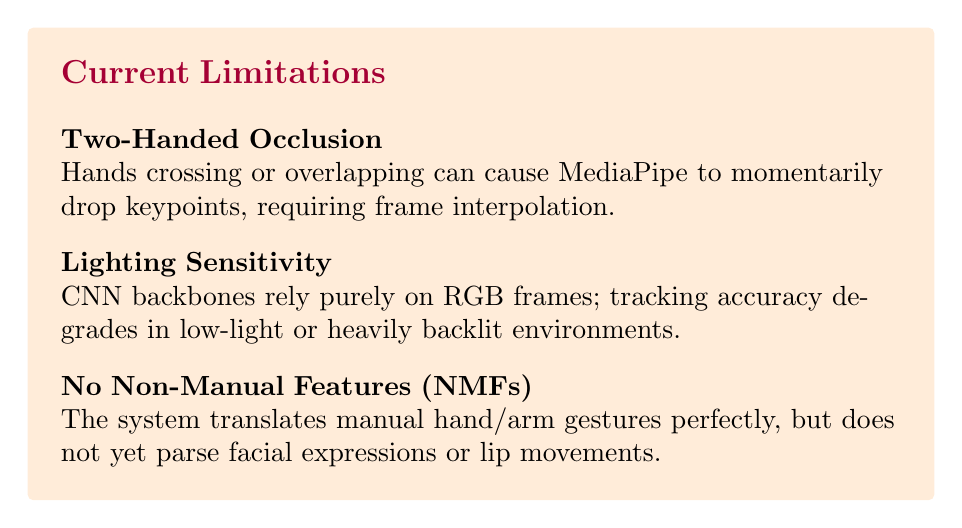
\begin{tikzpicture}
        \node[fill=orange!15, rounded corners=2pt, text width=0.88\textwidth, inner sep=12pt, align=left] {
            {\large \textbf{\textcolor{amritaMaroon}{Current Limitations}}}\\[4mm]
            
            \textbf{Two-Handed Occlusion}\\
            Hands crossing or overlapping can cause MediaPipe to momentarily drop keypoints, requiring frame interpolation.\\[3mm]
            
            \textbf{Lighting Sensitivity}\\
            CNN backbones rely purely on RGB frames; tracking accuracy degrades in low-light or heavily backlit environments.\\[3mm]
            
            \textbf{No Non-Manual Features (NMFs)}\\
            The system translates manual hand/arm gestures perfectly, but does not yet parse facial expressions or lip movements.
        };
    \end{tikzpicture}
\end{frame}

% ============================================================
% SLIDE 30: TEAM CONTRIBUTION MATRIX
% ============================================================
\section{Team Contribution}
\begin{frame}{30. Team Contribution}
    
    
    \vspace{2mm}
    \begin{center}
    \renewcommand{\arraystretch}{1.6} 
    {\fontsize{7pt}{9pt}\selectfont
    \begin{tabular}{|>{\raggedright\arraybackslash\bfseries}p{0.18\textwidth}|>{\raggedright\arraybackslash}p{0.36\textwidth}|>{\raggedright\arraybackslash}p{0.38\textwidth}|}
        \hline
        \rowcolor{maroon}
        \textcolor{white}{\textbf{Team Members}} & 
        \textcolor{white}{\textbf{Platform \& Application Work}} & 
        \textcolor{white}{\textbf{Sign Language Engine}} \\
        \hline
        
        Sai Sri Satvic L. \newline Vivin Rakul P. & 
        \textbf{Web Application Development}\newline
        $\bullet$ Built the web dashboard for uploading videos.\newline
        $\bullet$ Developed the real-time backend server.\newline
        $\bullet$ Integrated the 3D Avatar directly into the browser. & 
        \textbf{Two-Hand Movement \& Grammar}\newline
        $\bullet$ Designed logic to detect signs requiring both hands.\newline
        $\bullet$ Engineered the system to learn how gestures flow over time.\newline
        $\bullet$ Created grammar rules converting raw predictions into avatar instructions. \\
        \hline
        
        Snigdha Siri Valli A. \newline Vijay Saravana Pandi T. & 
        \textbf{Mobile Application Development}\newline
        $\bullet$ Designed the mobile app layout for smartphones.\newline
        $\bullet$ Built the camera module to capture live signs.\newline
        $\bullet$ Handled mobile app connectivity with the main server. & 
        \textbf{Single-Hand Movement \& Tracking}\newline
        $\bullet$ Developed the system to track single-handed signs.\newline
        $\bullet$ Built the feature that recognizes exact finger bending.\newline
        $\bullet$ Calculated the exact 3D spatial location and palm direction. \\
        \hline
    \end{tabular}
    }
    \end{center}
\end{frame}

% ============================================================
% SLIDE 31: REFERENCES
% ============================================================
\begin{frame}{31. References}
\scriptsize
\begin{enumerate}\setlength{\itemsep}{0.06cm}
\item S. Prillwitz et al., ``HamNoSys: Hamburg Notation System for Sign Languages,'' 1989.
\item D. Li et al., ``Word-level Deep Sign Language Recognition from Video (WLASL),'' \textit{Proc. WACV}, 2020.
\item C. Lugaresi et al., ``MediaPipe: A Framework for Building Perception Pipelines,'' \textit{Google Research}, 2019.
\item R. Kennaway, ``Synthetic animation of deaf signing gestures,'' \textit{Proc. GW 2001}, Springer, 2002.
\item V. Skobov, ``Direct Video-to-HamNoSys Translation Using CNN Features,'' 2020.
\item S. Stoll et al., ``Text2Sign: Towards Sign Language Production Using NMT,'' \textit{IJCV}, 2020.
\item J.~E.~Hopcroft, R.~Motwani, J.~D.~Ullman, ``Introduction to Automata Theory, Languages, and Computation,'' \textit{3rd ed., Pearson}, 2006.
\item A.~V.~Aho, M.~S.~Lam, M.~S.~Sethi, J.~D.~Ullman, ``Compilers: Principles, Techniques, and Tools (Dragon Book),'' \textit{2nd ed., Pearson}, 2006.
\item N.~Chomsky, ``Three Models for the Description of Language,'' \textit{IRE Transactions on Information Theory}, vol.~2, no.~3, pp.~113--124, 1956.
\item T.~Hanke, ``HamNoSys --- Representing Sign Language Data in Language Resources and Language Processing Contexts,'' \textit{Proc. LREC Workshop on Representation and Processing of Sign Languages}, 2004.
\end{enumerate}
\end{frame}

% ============================================================
% THANK YOU SLIDE
% ============================================================
\begin{frame}[plain]
\vspace*{\fill}
\centering

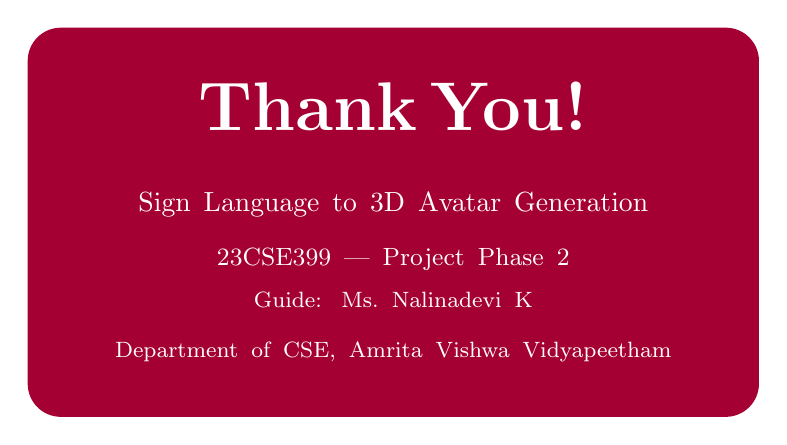
\begin{tikzpicture}
\node[
    fill=amritaMaroon,
    text=white,
    rounded corners=12pt,
    inner sep=20pt,
    text width=0.65\textwidth,
    align=center,
    font=\Large
] {
    \textbf{\Huge Thank You!}\\[6mm]
    \normalsize Sign Language to 3D Avatar Generation\\[3mm]
    \small 23CSE399 --- Project Phase 2\\[2mm]
    \footnotesize Guide: Ms.\ Nalinadevi K\\
    Department of CSE, Amrita Vishwa Vidyapeetham
};
\end{tikzpicture}

\vspace{8mm}
{\small\textcolor{darktext}{Questions \& Feedback Welcome}}

\vspace*{\fill}
\end{frame}

\end{document}
